% Options for packages loaded elsewhere
\PassOptionsToPackage{unicode}{hyperref}
\PassOptionsToPackage{hyphens}{url}
%
\documentclass[
]{article}
\usepackage{amsmath,amssymb}
\usepackage{iftex}
\ifPDFTeX
  \usepackage[T1]{fontenc}
  \usepackage[utf8]{inputenc}
  \usepackage{textcomp} % provide euro and other symbols
\else % if luatex or xetex
  \usepackage{unicode-math} % this also loads fontspec
  \defaultfontfeatures{Scale=MatchLowercase}
  \defaultfontfeatures[\rmfamily]{Ligatures=TeX,Scale=1}
\fi
\usepackage{lmodern}
\ifPDFTeX\else
  % xetex/luatex font selection
\fi
% Use upquote if available, for straight quotes in verbatim environments
\IfFileExists{upquote.sty}{\usepackage{upquote}}{}
\IfFileExists{microtype.sty}{% use microtype if available
  \usepackage[]{microtype}
  \UseMicrotypeSet[protrusion]{basicmath} % disable protrusion for tt fonts
}{}
\makeatletter
\@ifundefined{KOMAClassName}{% if non-KOMA class
  \IfFileExists{parskip.sty}{%
    \usepackage{parskip}
  }{% else
    \setlength{\parindent}{0pt}
    \setlength{\parskip}{6pt plus 2pt minus 1pt}}
}{% if KOMA class
  \KOMAoptions{parskip=half}}
\makeatother
\usepackage{xcolor}
\usepackage[margin=1in]{geometry}
\usepackage{longtable,booktabs,array}
\usepackage{calc} % for calculating minipage widths
% Correct order of tables after \paragraph or \subparagraph
\usepackage{etoolbox}
\makeatletter
\patchcmd\longtable{\par}{\if@noskipsec\mbox{}\fi\par}{}{}
\makeatother
% Allow footnotes in longtable head/foot
\IfFileExists{footnotehyper.sty}{\usepackage{footnotehyper}}{\usepackage{footnote}}
\makesavenoteenv{longtable}
\usepackage{graphicx}
\makeatletter
\def\maxwidth{\ifdim\Gin@nat@width>\linewidth\linewidth\else\Gin@nat@width\fi}
\def\maxheight{\ifdim\Gin@nat@height>\textheight\textheight\else\Gin@nat@height\fi}
\makeatother
% Scale images if necessary, so that they will not overflow the page
% margins by default, and it is still possible to overwrite the defaults
% using explicit options in \includegraphics[width, height, ...]{}
\setkeys{Gin}{width=\maxwidth,height=\maxheight,keepaspectratio}
% Set default figure placement to htbp
\makeatletter
\def\fps@figure{htbp}
\makeatother
\setlength{\emergencystretch}{3em} % prevent overfull lines
\providecommand{\tightlist}{%
  \setlength{\itemsep}{0pt}\setlength{\parskip}{0pt}}
\setcounter{secnumdepth}{5}
\ifLuaTeX
  \usepackage{selnolig}  % disable illegal ligatures
\fi
\IfFileExists{bookmark.sty}{\usepackage{bookmark}}{\usepackage{hyperref}}
\IfFileExists{xurl.sty}{\usepackage{xurl}}{} % add URL line breaks if available
\urlstyle{same}
\hypersetup{
  pdftitle={TSMC Revenue Forecasting using Time Series Analysis},
  pdfauthor={Rohit Jangid, Gaurish Bansal},
  hidelinks,
  pdfcreator={LaTeX via pandoc}}

\title{TSMC Revenue Forecasting using Time Series Analysis}
\author{Rohit Jangid, Gaurish Bansal}
\date{2023-07-08}

\begin{document}
\maketitle

{
\setcounter{tocdepth}{2}
\tableofcontents
}
\hypertarget{abstract}{%
\section{Abstract}\label{abstract}}

This project presents an analysis of the monthly revenue of Taiwanese
Semiconductor Manufacturing Company (TSMC) using time series models.
Specifically, three different models, namely SARIMA, Holt-Winters, and
FB Prophet, were compared to determine their forecasting performance.
Evaluation metrics such as Mean Absolute Error (MAE), Root Mean Square
Error (RMSE), Mean Absolute Percentage Error (MAPE), and Mean Absolute
Scaled Error (MASE) were employed for model comparison. The objective
was to select the best-performing model based on these metrics and
provide an accurate revenue forecast for the next quarter. The analysis
began with a comprehensive exploration of TSMC's monthly revenue data,
examining trends, seasonality, and other patterns that could impact
revenue. Subsequently, the SARIMA, Holt-Winters, and FB Prophet models
were trained using historical revenue data. The performance of each
model was evaluated using the aforementioned metrics, enabling the
assessment of accuracy and robustness in capturing revenue patterns. By
comparing the results, the model that yielded the most accurate
forecasts for TSMC's revenue was the SARIMA model. The selected model
was then used to forecast revenue for the upcoming year, providing
valuable insights for stakeholders such as investors, analysts, and
decision-makers. The research paper also highlights the strengths and
limitations of each model, contributing to the field of time series
analysis and offering a foundation for further research in revenue
forecasting and related domains.

\hypertarget{introduction}{%
\section{Introduction}\label{introduction}}

The ability to accurately forecast revenue is of utmost importance for
companies seeking to make informed business decisions, plan strategies,
and meet financial objectives. Time series analysis provides a valuable
framework for understanding and predicting patterns in sequential data,
making it a suitable approach for revenue forecasting. In this project
paper, we focus on the monthly revenue of Taiwanese Semiconductor
Manufacturing Company (TSMC) and aim to compare the forecasting
performance of three popular time series models: SARIMA, Holt-Winters,
and FB Prophet.

The first step in our analysis involves an exploration of TSMC's monthly
revenue data, obtained from TSMC's website. This exploration aims to
identify any underlying trends, seasonality, or other patterns that
might influence the revenue. By understanding these patterns, we can
better select and evaluate appropriate models for revenue forecasting.

We then proceed to train the SARIMA, Holt-Winters, and FB Prophet models
using the available historical revenue data. These models are widely
used in time series analysis and offer different approaches for
capturing the dynamics of revenue patterns. To compare their
performance, we employ evaluation metrics such as Mean Absolute Error
(MAE), Root Mean Square Error (RMSE), Mean Absolute Percentage Error
(MAPE), and Mean Absolute Scaled Error (MASE). These metrics allow us to
assess the accuracy and robustness of each model in capturing revenue
patterns and make an informed selection of the best-performing model.

Upon identifying the best model, we utilize it to forecast TSMC's
revenue for the next quarter. This forecast provides valuable insights
for stakeholders, including investors, analysts, and decision-makers,
enabling them to gain a better understanding of TSMC's future financial
performance. The findings of our study can aid in making informed
decisions regarding TSMC's financial strategies and serve as a
foundation for further research in the domain of time series
forecasting.

\begin{longtable}[]{@{}
  >{\raggedright\arraybackslash}p{(\columnwidth - 6\tabcolsep) * \real{0.2466}}
  >{\raggedright\arraybackslash}p{(\columnwidth - 6\tabcolsep) * \real{0.2466}}
  >{\raggedright\arraybackslash}p{(\columnwidth - 6\tabcolsep) * \real{0.2603}}
  >{\raggedright\arraybackslash}p{(\columnwidth - 6\tabcolsep) * \real{0.2466}}@{}}
\caption{Outline and proceedings of the project.}\tabularnewline
\toprule\noalign{}
\begin{minipage}[b]{\linewidth}\raggedright
Date
\end{minipage} & \begin{minipage}[b]{\linewidth}\raggedright
Objective
\end{minipage} & \begin{minipage}[b]{\linewidth}\raggedright
Outcome
\end{minipage} & \begin{minipage}[b]{\linewidth}\raggedright
Delegated Tasks
\end{minipage} \\
\midrule\noalign{}
\endfirsthead
\toprule\noalign{}
\begin{minipage}[b]{\linewidth}\raggedright
Date
\end{minipage} & \begin{minipage}[b]{\linewidth}\raggedright
Objective
\end{minipage} & \begin{minipage}[b]{\linewidth}\raggedright
Outcome
\end{minipage} & \begin{minipage}[b]{\linewidth}\raggedright
Delegated Tasks
\end{minipage} \\
\midrule\noalign{}
\endhead
\bottomrule\noalign{}
\endlastfoot
06-05-2023 & Plan a timeline and set a schedule and decide company & We
will be applying the principles of time series analysis to understand
the revenue of TSMC & Read an example research paper (TSA of Jute
demand) and collect the revenue data of TSMC \\
10-05-2023 & Discuss the research paper & Built an understanding of how
research is done & Make a list of TS models which could be used. \\
15-05-2023 & Discuss potential TS models & One modern model will be
compared against classical models & List down the Advantages,
disadvantages, and use cases for each model. Find customers of TSMC \\
18-05-2023 & Discuss the collected model's & Classical models finalized
- Seasonal ARIMA and Exponential Smoothing models & Collect the data
regarding companies that buy from TSMC \\
23-05-2023 & Finalize the modern model & LSTM model finalized & Find
appropriate determinants for comparison between models and read a case
study for LSTM \\
26-05-2023 & Discuss the LSTM case study and possible determinants &
RMSE, MAE, MAPE, and MASE will be used to compare models while AICc
value will be used to select the parameters & Implement the Seasonal
ARIMA models and the ES models. \\
29-05-2023 & Discuss the Classical models' fit and share some plots &
Log{[}revenue{]} will be used for analysis & Calculate AICc values and
finalize model parameters in SARIMA models and ES models \\
02-06-2023 & Discuss the final two models & Finalized -
SARIMA{[}4,1,1{]}{[}1,0,2{]}{[}12{]} and Holt Winters' Additive Model &
Implement LSTM Model \\
05-06-2023 & Discuss LSTM & The LSTM model does not fit well & Try to
make a better LSTM model and find another modern model \\
12-06-2023 & Discuss changing the model & Discarded LSTM model and
presented the Prophet model & Read about the prophet model and find case
studies implementing this model in the field of finance \\
15-06-2023 & Discuss the case studies & More study required before
implementing this model & List down the problems in the LSTM model and
how can the Prophet model be better \\
19-06-2023 & Discuss more case studies and finalize the model &
Finalized the Prophet model & Implement the prophet model and read the
history of TSMC company \\
22-06-2023 & Discuss CV techniques & Cross-Validation using the Rolling
Origin method will be used & Implement Cross-Validation and compare the
models \\
26-06-2023 & Share the results of the CV & The prophet model is the best
& Make a report draft and considered publishing our results \\
04-07-2023 & Share the final Report & Made important changes to the
report & Submit the supplementary folder with the final report \\
\end{longtable}

\hypertarget{literature-review}{%
\section{Literature Review}\label{literature-review}}

The field of forecasting in various industries has seen significant
advancements in recent years, with researchers exploring different
quantitative models and techniques to improve the accuracy and
reliability of predictions. Four research papers contribute to this
field by focusing on different aspects of forecasting and evaluating the
performance of various models.

In 2016 Jana Fabianová*, Peter Kačmáry, Vieroslav Molnár, and Peter
Michalik\(^{[2]}\) focused on addressing data uncertainty in sales
forecasting. The researchers utilized historical data, probabilistic
modeling techniques, and the SARIMA model to generate realistic and
robust sales forecasts. By considering data uncertainty, the tool
enhanced forecast accuracy and aided in decision-making processes by
providing a range of potential outcomes. This study highlighted the
advantages of incorporating data uncertainty in sales forecasting and
demonstrates the effectiveness of probabilistic modeling techniques. In
2017, C. L. Karmaker, P. K. Halder and E. Sarker\(^{[1]}\) investigated
the application of quantitative forecasting models for predicting the
demand for jute yarn. By comparing models such as simple moving average,
single exponential, double exponential (Holt's), Winters, and
decomposition methods, the researchers aimed to determine the most
effective model. They evaluated the models using error determinants like
mean absolute deviation (MAD), mean absolute percentage error (MAPE),
and mean square deviation (MSD). The study provided a comprehensive
analysis of these models on a weekly basis over a four-year period,
allowing for a detailed examination of their forecasting performance. In
2017 Serkan ARAS , İpek DEVECİ KOCAKOÇ, and Cigdem POLAT\(^{[3]}\)
presented a comparative study of single and combination forecasting
methods for predicting retail sales. Various forecasting methods,
including time series models, regression analysis, and machine learning
algorithms, were applied to historical sales data. Statistical tests,
model selection using the Akaike Information Criterion corrected (AICc),
and residual analysis were employed to evaluate and compare the
forecasting methods. The study provided insights into the strengths and
limitations of both single and combination methods in the context of
retail sales forecasting, using appropriate error metrics for
performance evaluation.Finally in 2020, Emir Žunić, Kemal Korjenić,
Kerim Hodžić and Dženana Đonko\(^{[4]}\) focused on the application of
Facebook's Prophet algorithm for accurate sales forecasting based on
real-world data. The researchers employed the Prophet algorithm, which
handles time series forecasting with seasonality and trends. The
algorithm captured different components of the sales data and generated
probabilistic forecasts with uncertainty intervals. The study showcased
the algorithm's capabilities in handling complex time series patterns
and provided insights into its performance using error metrics. It
emphasized the algorithm's practicality and potential benefits for
businesses in terms of improved decision-making and resource allocation.

Overall, these four papers contributed to the field of forecasting by
evaluating different quantitative models and techniques for various
industries. They highlighted the importance of accurate forecasting in
optimizing business processes and decision-making. The studies
emphasized the need to consider data uncertainty, evaluate multiple
models, and employ appropriate error metrics for performance evaluation.
Our study draws inspiration from these research papers to add valuable
insights and practical guidance for researchers and practitioners in the
field of forecasting

\hypertarget{methodology}{%
\section{Methodology}\label{methodology}}

We begin by reviewing the basics of time series analysis and create a
basis for understanding the various times series models used in this
project.

\hypertarget{time-series-analysis}{%
\subsection{Time Series Analysis}\label{time-series-analysis}}

A time series is a collection of observations or data points measured
and recorded sequentially over regular time intervals. Formally, a time
series can be defined as an ordered sequence of data points represented
as Yt, where t denotes the time index and Yt represents the observed
value or measurement at a time ``t''. The time series data can be
discrete or continuous, depending on the nature of the variable being
measured.

In a time series, the observations are typically recorded at equidistant
time intervals, such as hourly, daily, monthly, or yearly. The data
points are often influenced by various factors, including seasonality,
trends, cyclic patterns, and random fluctuations. These characteristics
make time series analysis a valuable tool for understanding and
predicting future behaviour based on past patterns and trends.

Time series analysis involves studying the properties, patterns, and
dynamics of the data, as well as developing mathematical models and
statistical techniques to capture and explain its behaviour.

\hypertarget{definitions}{%
\subsection{Definitions}\label{definitions}}

\begin{enumerate}
\def\labelenumi{\arabic{enumi}.}
\tightlist
\item
  \emph{Data Point}: A data point refers to a single observation or
  measurement recorded at a specific time point in a time series.
\item
  \emph{Time Interval}: A time interval is a duration between successive
  time points or observations in a time series. It represents the
  granularity or frequency at which the data is collected or recorded.
\item
  \emph{Lag}: Lag refers to the time distance between two observations
  in a time series.
\item
  \emph{Autocorrelation}: Autocorrelation measures the linear
  relationship between the values of a variable in a time series at
  different time lags. It helps identify the presence of any serial
  dependence or correlation between observations.
\item
  \emph{Autocorrelation function (ACF)}: ACF measures the linear
  dependence between an observation and its lagged values. The ACF plots
  shows autocorrelation coefficients at different lags, indicating how
  past values at those lags can predict future values.
\item
  \emph{Partial autocorrelation function (PACF)}: PACF measures the
  direct relationship between an observation and its lagged values while
  considering intermediate lags. The PACF plots shows partial
  autocorrelation coefficients at various lags, revealing significant
  direct relationships without the influence of intervening lags.
\item
  \emph{Unit root}: A unit root in a time series refers to a
  characteristic where the series exhibits a random trend and does not
  revert to a constant mean over time. In other words, the series does
  not show a tendency to converge towards a specific average value or
  exhibit stationarity.
\item
  \emph{Forecasting}: Forecasting involves predicting or estimating
  future values or patterns of a variable in a time series based on
  historical data. It aims to capture and project the underlying
  behaviour and trends in the data.
\item
  \emph{Forecast Horizon}: Refers to the time duration into the future
  for which predictions are generated in a time series analysis. It
  indicates the length of the forecasted values beyond the present or
  the last observed data point and helps determine the timeframe for
  decision-making and planning based on the forecasted information.
\item
  \emph{Homoscedasticity}: Homoscedasticity refers to the property of a
  time series where the variance of the errors or residuals remains
  constant or consistent across different time periods i.e.~the
  variability of the data points in the series does not change
  systematically over time.
\end{enumerate}

\hypertarget{components-of-a-time-series}{%
\subsection{Components of a Time
Series}\label{components-of-a-time-series}}

In time series analysis, a series is often decomposed into several
components that collectively capture the different patterns and
variations present in the data. The main components of a time series
are:~

\begin{enumerate}
\def\labelenumi{\arabic{enumi}.}
\tightlist
\item
  \emph{Trend}: The trend component represents the long-term pattern or
  direction of the data. It indicates whether the variable is
  increasing, decreasing, or following a relatively stable pattern over
  time. The trend can be linear, nonlinear, or even non-existent.
\item
  \emph{Seasonality}: Seasonality refers to the repetitive and
  predictable patterns that occur within a time series at regular
  intervals, typically within a year or a shorter period. These patterns
  may be influenced by seasonal factors, such as weather, holidays, or
  economic cycles. Seasonality can be additive or multiplicative,
  depending on whether the magnitude of the seasonal pattern remains
  constant or varies with the level of the series.~
\item
  \emph{Cyclical} \emph{patterns}: The cyclical component captures the
  irregular patterns or fluctuations in a time series that are not of
  fixed period or related to specific calendar effects. These cycles are
  typically longer than the seasonal cycles and can be influenced by
  economic, business, or geopolitical factors. Cyclical patterns are
  often associated with boom and bust cycles, but their duration and
  magnitude can vary.~
\item
  \emph{Irregularity} or \emph{Residual}: The irregular component, also
  referred to as the residual or error component, represents the random
  or unpredictable fluctuations that cannot be explained by the other
  components. It encompasses any noise, randomness, or unexplained
  variation in the time series data.
\item
  \emph{Level}: Level refers to the underlying or average behaviour of
  the data over time, which is often incorporated into the trend
  component and is not typically considered a distinct component of a
  time series.
\end{enumerate}

\hypertarget{stationarity}{%
\subsection{Stationarity}\label{stationarity}}

Stationarity is a property of a time series where the statistical
properties, such as mean, variance, and covariance, remain constant over
time. A stationary time series exhibits stable behaviour and is often
easier to model and analyse compared to non-stationary series.~

Here are some key reasons why stationarity is desirable:

\begin{enumerate}
\def\labelenumi{\arabic{enumi}.}
\tightlist
\item
  Simplified Modelling: Stationary time series exhibit consistent
  statistical properties over time, such as constant mean, constant
  variance, and autocovariance that depends only on the time lag. This
  simplifies the modelling process by allowing us to assume that the
  statistical properties of the data remain constant throughout the
  series. Modelling a stationary series is often easier and more
  straightforward compared to non-stationary series.
\item
  Predictability: Stationary time series exhibit stable and predictable
  behaviour. The patterns observed in the past are likely to persist in
  the future, making it easier to forecast future values based on
  historical data. Stationary series allow for reliable extrapolation
  and forecasting using mathematical models, such as autoregressive
  integrated moving average (ARIMA)
\item
  Interpretability: Stationarity enables the identification and
  interpretation of the underlying patterns and dynamics within a time
  series. By removing trends and seasonality through differencing or
  other transformations, the focus can be shifted to the cyclical or
  residual components, allowing for a better understanding of the true
  underlying behaviour of the data.
\end{enumerate}

\textbf{Tests for checking stationarity}

When a time series has a unit root, it implies that the series is
non-stationary, and its statistical properties, such as mean and
variance, are not constant over time. Instead, the series may exhibit
trends, cycles, or other patterns that can make it challenging to
analyze or model accurately.

\begin{enumerate}
\def\labelenumi{\arabic{enumi}.}
\item
  \emph{Augmented Dickey-Fuller (ADF) Test}: The ADF test is a widely
  used test for stationarity. It assesses whether a unit root is present
  in a time series, indicating non-stationarity. The null hypothesis of
  the test is that the series has a unit root (i.e., it is
  non-stationary). If the p-value associated with the ADF test is below
  a chosen significance level (e.g., 0.05), the null hypothesis is
  rejected, indicating stationarity.
\item
  \emph{Kwiatkowski-Phillips-Schmidt-Shin (KPSS) Test}: The KPSS test is
  another commonly employed test for stationarity. It examines whether a
  time series is trend-stationary or difference-stationary. The null
  hypothesis of the KPSS test is that the series is trend-stationary. If
  the p-value is above a specified significance level, the null
  hypothesis is not rejected, indicating stationarity.
\end{enumerate}

\textbf{Methods to make time series stationary}

To make a time series stationary, you can employ various methods and
transformations. The specific approach you choose depends on the
characteristics of the data and the nature of the non-stationarity. Here
are some common methods for making a time series stationary:~

\begin{enumerate}
\def\labelenumi{\arabic{enumi}.}
\tightlist
\item
  \emph{Differencing}: Differencing involves taking the difference
  between consecutive observations in the time series. This method is
  effective for removing a trend or linear component. If the series
  exhibits a constant growth rate, you can apply first-order
  differencing (subtracting each observation from its previous
  observation). For higher-order differencing, you can repeat the
  differencing process multiple times until the series becomes
  stationary.~
\item
  \emph{Logarithmic} \emph{transformation}: If the series displays
  exponential growth or varying variance over time, applying a
  logarithmic transformation can stabilise the variance and make the
  series more stationary. Taking the natural logarithm of the series
  values helps in reducing the magnitude of large values and dampening
  the exponential growth.
\item
  \emph{Seasonal} \emph{differencing}: Seasonal differencing involves
  taking the difference between observations at a fixed seasonal
  interval. This method is useful for removing seasonal patterns or
  periodic fluctuations. By subtracting the observation from the
  corresponding observation in the previous season, you can eliminate
  the seasonal component and potentially achieve stationarity.~
\item
  \emph{Miscellaneous} \emph{transformation} \emph{techniques}: Certain
  mathematical transformations can help stabilize the variance of a time
  series. For example, the Box-Cox transformation can be applied to
  handle cases where the variance of the series changes with the level.
  This transformation applies a power function to the series, allowing
  for different types of transformations depending on the chosen
  parameter \(\lambda\).
\end{enumerate}

The choice of method depends on the specific characteristics and
behaviour of the time series. Additionally, after applying the
transformation or differencing, it is crucial to assess the stationarity
of the resulting series using statistical tests, such as the Augmented
Dickey-Fuller (ADF) test.

\hypertarget{residuals}{%
\subsection{Residuals}\label{residuals}}

Residuals are the differences between the observed values of a time
series and the corresponding predicted values from a forecasting model.
Residuals are an essential component in time series analysis and
modelling.

\textbf{Properties of Residuals}

\begin{enumerate}
\def\labelenumi{\arabic{enumi}.}
\item
  \emph{Mean} \emph{Zero}: The residuals should have an average value
  close to zero. A non-zero mean may indicate a systematic bias in the
  model.
\item
  \emph{Independence}: Residuals should be independent of each other.
  Autocorrelation in residuals suggests that the model fails to capture
  the temporal dependencies in the data.
\item
  \emph{Homoscedasticity}: Residuals should exhibit constant variance
  over time. Heteroscedasticity, where the variance of residuals varies
  with the level of the series, may indicate model inadequacy.
\item
  \emph{Normally} \emph{Distributed}: Residuals should follow a normal
  distribution. Departure from normality may affect the validity of
  statistical inference and prediction intervals.
\end{enumerate}

\textbf{Ljung-Box test}

The Ljung-Box test examines the presence of autocorrelation in the
residuals. If the test results indicate significant autocorrelation, it
suggests that the model may need further refinement or consideration of
additional explanatory variables.

The Ljung--Box test is defined as:

\(H_0\) : The data are independently distributed (i.e.~the correlations
in the population from which the sample is taken are 0, so that any
observed correlations in the data result from randomness of the sampling
process).

\(H_a\): The data are not independently distributed; they exhibit serial
correlation.

The test statistic is
\[Q=n(n+2) \sum_{k=1}^{h}{\frac{\sigma_k^2}{n-k}}\] where \(n\) is the
sample size \(\sigma_k\) is the sample autocorrelation at lag \(k\),and
\(h\) is the number of lags being tested. Under \(H_0\) the statistic
\(Q\) asymptotically follows a \(χ^{2}_{h}\). For significance level
\(\alpha\), the critical region for rejection of the hypothesis of
randomness is \[Q>\chi^2_{1-\alpha,h}\] where \(\chi^2_{1-\alpha,h}\) is
the \((1 − \alpha)\)-quantile of the chi-squared distribution with \(h\)
degrees of freedom. The Ljung--Box test is commonly used in
autoregressive integrated moving average (ARIMA) modelling. When testing
the residuals of an estimated ARIMA model, the degrees of freedom need
to be adjusted to reflect the parameter estimation. For example, for
an\(ARIMA(p, 0, q)\) model, the degrees of freedom should be set to
\(h-p-q\).

\hypertarget{determinants-and-information-criteria}{%
\subsection{Determinants and Information
Criteria}\label{determinants-and-information-criteria}}

Errors in time series forecasting refer to the differences between the
predicted values and the actual observed values of the time series.
Errors provide a direct evaluation of the forecasting accuracy and help
assess the performance of different forecasting models. Lower error
values indicate better accuracy and closer alignment with the actual
data.

Information criteria, such as the Akaike Information Criterion (AIC) and
the Bayesian Information Criterion (BIC), are statistical measures used
to compare and select between different competing models. These criteria
aim to balance the goodness of fit of the model with the complexity or
number of parameters used in the model. Information criteria penalise
models with a higher number of parameters, encouraging parsimony and
avoiding overfitting. The lower the information criterion value, the
better the trade-off between model fit and complexity.

Some commonly used errors and information criteria are:

\begin{description}
\item[1. RMSE]
It provides a measure of the standard deviation of the forecast errors
and is sensitive to larger
errors.\[ \sqrt{\frac{1}{n} \sum_{i=1}^{n}{(Y_i - \hat{Y_i})^2}} \]
\item[2. MAE]
It gives an indication of the average magnitude of the forecast errors
in the original scale of the data.

\[ \frac{1}{n}\sum_{i=1}^{n}{|Y_i-\hat{Y}_i|} \]
\item[3. MAPE]
It provides an understanding of the average magnitude of the forecast
errors relative to the actual values.

\[ \frac{1}{n}\sum_{i=1}^{n}{\frac{Y_i-\hat{Y_i}}{Y_i}\cdot100} \]
\item[4. MASE]
It provides a relative measure of accuracy, which is helpful when
comparing forecast performance across different time
series.\[ \frac{1}{n}\sum_{i=1}^{n}{\frac{|Y_i-\hat{Y_i}|}{\frac{1}{T-m}\sum_{t=m+1}^{n}|Y_t-Y_{t-m}|}} \]
\item[5. AIC]
Given a collection of models for the data, AIC estimates the quality of
each model, relative to each of the other models. Thus, AIC provides a
means for model selection.\[ 2k-\log(L(\theta)) \]
\item[6. AICc]
It is equal to AIC with a correction for small sample sizes. The formula
for AICc depends upon the statistical model. Assuming that the model is
univariate, is linear in its parameters, and has normally-distributed
residuals (conditional upon regressors), then the formula for AICc is as
follows. \[AICc  = AIC + \frac{2k^2+2k}{n-k-1} \]
\item[7. BIC]
It generally penalizes free parameters more strongly than the AIC,
though it depends on the size of \(n\) and relative magnitude of \(n\)
and \(k\). \[k\ln(n) - 2\log(L(\theta))\]
\end{description}

where \(n\) denotes the sample size, \(Y_i\) denotes the \(i^{th}\)
timestamp, \(\hat{Y_i}\) denotes the forcast for the \(i^{th}\)
timestamp, \(m\) denotes the seasonal period, \(k\) denotes the number
of parameters in the model and \(L(\theta)\) denotes the likelihood of
the model.

\hypertarget{cross-validation}{%
\subsection{Cross Validation}\label{cross-validation}}

Cross-validation is a technique used to evaluate the performance and
generalise the effectiveness of a predictive model. It involves
partitioning the available dataset into subsets, typically a training
set and a validation set, and iteratively training and evaluating the
model on different combinations of these subsets.~

The basic steps of cross-validation are as follows:~

\begin{enumerate}
\def\labelenumi{\arabic{enumi}.}
\item
  Splitting the dataset: The original dataset is divided into k subsets
  or folds of approximately equal size.~
\item
  Model training and evaluation: The model is trained on k-1 folds of
  the data, and the remaining fold is used for validation. This process
  is repeated k times, with each fold serving as the validation set
  once.~
\item
  Performance metrics: The performance of the model is assessed on each
  validation set, and the evaluation results (such as accuracy, mean
  squared error, or other relevant metrics) are recorded.~
\item
  Aggregating results: The performance metrics from each iteration are
  averaged or combined to obtain an overall assessment of the model's
  performance.~
\end{enumerate}

The main purpose of cross-validation is to estimate how well a model
will perform on unseen data. It helps to assess the model's ability to
generalise and identifies potential issues such as overfitting or
underfitting. By using different subsets of the data for training and
validation, cross-validation provides a more robust evaluation of the
model's performance compared to a single train-test split.~

Commonly used cross-validation methods include k-fold cross-validation,
stratified k-fold cross-validation, leave-one-out cross-validation, and
holdout validation. The choice of the cross-validation method depends on
the size of the dataset, the nature of the problem, and other
considerations.

In this study, We are using a rolling origin Method for cross validation

Rolling origin cross-validation, also known as rolling window or sliding
window cross-validation, is a variation of the traditional
cross-validation technique. It is commonly used in time series analysis
and forecasting to assess the performance of predictive models on
sequential data.~

In rolling origin cross-validation, a fixed-size training window is
defined, and the model is trained on the observations within this
window. The model is then tested on the next observation that
immediately follows the training window, which serves as the validation
or test set. This process is repeated by sliding the window one step
forward and retraining the model, generating new predictions and
evaluating their performance at each step. Figure 1 shows a visual
representation of this method.

The main steps involved in rolling origin cross-validation are as
follows:~

\begin{enumerate}
\def\labelenumi{\arabic{enumi}.}
\item
  Set the initial training window: Determine the size of the training
  window, which typically consists of a fixed number of sequential
  observations.~
\item
  Train and evaluate the model: Train the model on the data within the
  training window. Use the model to make predictions for the next
  observation in the sequence, which serves as the validation set.
  Evaluate the performance of the model based on the prediction accuracy
  or relevant metrics.~
\item
  Slide the window: Move the training window one step forward by
  removing the earliest observation and including the next observation
  in the sequence. Retrain the model using the updated training window,
  make predictions for the next observation, and evaluate the model's
  performance again.~
\item
  Repeat the process: Repeat steps 2 and 3 until the training window
  reaches the end of the available data, generating predictions and
  performance evaluations at each step.~
\end{enumerate}

Rolling origin cross-validation allows for the assessment of a model's
performance on sequential data, which is crucial in time series analysis
and forecasting. It provides a more realistic evaluation of the model's
ability to generalise to future observations by simulating the
real-world forecasting scenario where the model is updated and retrained
as new data becomes available. This approach helps to capture changes in
the underlying patterns or dynamics of the time series over time and
provides a more accurate representation of the model's performance
compared to traditional cross-validation methods that assume independent
and identically distributed samples.

\begin{figure}
\centering
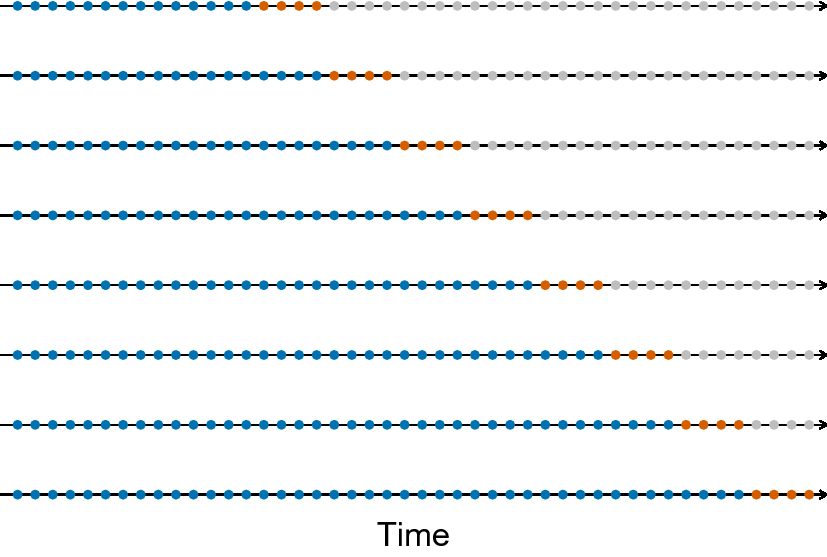
\includegraphics[width=10.61458in,height=3.90625in]{Plots/rolling-origin-cross-validation.png}
\caption{Schematic representation of rolling origin method for cross
validation}
\end{figure}

\hypertarget{models}{%
\subsection{Models}\label{models}}

Although there are many models which are used in time series analysis,
this project mainly focuses on the most popular ones (SARIMA and
Holt-Winters) and the most recent ones ( FB Prophet)

\hypertarget{naive-model}{%
\subsubsection{Naive Model}\label{naive-model}}

The naive model is one of the simplest and most basic approaches for
time series forecasting. It assumes that the future values of a time
series will be the same as the most recent observed value. In other
words, the naive model assumes that there is no trend, seasonality, or
any other pattern in the data, and the future values will simply be a
repetition of the last observed value.

The naive model is straightforward and quick to implement, but it is
highly simplistic and assumes that the future behaviour of the time
series will be the same as the most recent observation. It doesn't
account for any underlying patterns, trends, or seasonality in the data,
so its accuracy is often limited. However, it can serve as a baseline
model for comparison against more sophisticated forecasting methods.

Equation: \[ Y_{t}\ = \ Y_{t - 1}\ \]

\hypertarget{arima}{%
\subsubsection{ARIMA}\label{arima}}

ARIMA is a class of models which was developed by combing the smaller
and simpler models togather.

\hypertarget{autoregressive-ar}{%
\paragraph{Autoregressive (AR)}\label{autoregressive-ar}}

The AR model assumes that the current value of a variable is a linear
combination of its previous values and a random error term.

We refer to the following equation as the \(AR(p)\) modelan
autoregressive Model of order \(p\), where \(p\) determines the number
of lagged terms considered in the model.

\(Y_{t} = c + \phi_{1}Y_{t - 1} + \phi_{2}Y_{t - 2} + \cdots +\)
\(\ \phi_{p}Y_{t - p} + \varepsilon_{t} ,\ \varepsilon_{t}\text{ is white noise.}\)

Parameter Constraints for stationary data for an \(AR(1)\) model
\(-1<\phi_{1}<1\) . For an \(AR(2)\) model \(− 1 < \phi_{2} < 1\),
\(\phi_{1}+ \phi_{2}<1 , \phi_{2} − \phi_{1}<1\)

\hypertarget{moving-average-ma}{%
\paragraph{Moving Average (MA)}\label{moving-average-ma}}

A moving average model forecasts the future values of a time series
based on the weighted average of past error terms. It assumes that the
current value of the series depends on the past error terms and a random
error term. The order of the moving average model, denoted as \(MA(q)\),
specifies the number of lagged error terms considered in the model.

\(Y_{t} = c + \varepsilon_{t} + \theta_{1}\varepsilon_{t - 1} + \theta_{2}\varepsilon_{t - 2} + \cdots\)
\(\theta_{q}\ \varepsilon_{t - q}\ ,\ \varepsilon_{t}\ \text{is white noise.}\)

Parameter Constraints for stationary data for an \(MA(1)\) model is
\(-1<\theta_{1}<1\) and for an \(MA(2)\) model is \(-1<\theta_{1}<1\),
\(\theta_{1}\) \(+\theta_{2}<1\) , \(\theta_{2}\) \(-\theta_{1}<1\).

It is important to note that the MA model assumes stationarity of the
time series, meaning that the mean and variance of the series remain
constant over time. If the time series exhibits non-stationarity,
pre-processing techniques such as differencing can be applied to make it
stationary before fitting the MA model.

\hypertarget{autoregressive-moving-average-arma}{%
\paragraph{Autoregressive Moving Average
(ARMA)}\label{autoregressive-moving-average-arma}}

The ARMA (Autoregressive Moving Average) model is a popular time series
model that combines the autoregressive (AR) and moving average (MA)
components to capture both the linear dependence on past values and the
influence of past error terms.

The full \(ARMA(p,q)\) can be written as:

\(p\) = order of the autoregressive component, specifying the number of
lagged terms of the dependent variable included in the model.

\(q\) = order of the moving average component, specifying the number of
lagged error terms included in the model.

\(Y_{t} = c + \phi_{1}Y_{t - 1} + \phi_{2}Y_{t - 2} + \cdots\  +\)
\(\phi_{p}Y_{t - p} + \varepsilon_{t} + \theta_{1}\varepsilon_{t - 1} + \theta_{2}\varepsilon_{t - 2} + \cdots\ \theta_{q}\varepsilon_{t - q}\)

\hypertarget{autoregressive-integrated-moving-average-arima}{%
\paragraph{Autoregressive Integrated Moving Average
(ARIMA)}\label{autoregressive-integrated-moving-average-arima}}

The ARIMA model incorporates the autoregressive component (AR) to
capture the linear dependence on past values, the differencing component
(I) to achieve stationarity, and the moving average component (MA) to
capture the influence of past error terms.

The full \(ARIMA (p,d,q)\) model can be written as:

\(Y'_{t} = c + \phi_{1}{Y'}_{t - 1} + \phi_{2}{Y'}_{t - 2} + \cdots\  + \phi_{p}{Y'}_{t - p} + \varepsilon_{t} + \theta_{1}\varepsilon_{t - 1} + \theta_{2}\varepsilon_{t - 2} + \  \cdots \  + \theta_{q}\varepsilon_{t - q}\)

\({Y'}_{t}\) is the differenced series.

\(p\) and \(q\) are order of the autoregressive component and order of
the moving average component respectively.

\(d\) = degree of differencing, indicating the number of times the data
needs to be differenced to achieve stationarity.

\hypertarget{seasonal-autoregressive-integrated-moving-average-sarima}{%
\paragraph{Seasonal Autoregressive Integrated Moving Average
(SARIMA)}\label{seasonal-autoregressive-integrated-moving-average-sarima}}

The SARIMA model is an extension of the ARIMA model that incorporates
seasonal patterns in time series data. It is used to capture both the
non-seasonal and seasonal components of a time series.

The SARIMA model is denoted as \(SARIMA(p, d, q)(P, D, Q)[m]\), where
\(p,\ d,\ q,\ P,\ D,\ Q, \text{ and }m\) represents the order of the
non-seasonal autoregressive component, the degree of non-seasonal
differencing, the order of the non-seasonal moving average component,
the order of the seasonal autoregressive component, the degree of
seasonal differencing, the order of the seasonal moving average
component, and the length of the seasonal cycle respectively.

\hypertarget{exponential-smoothing}{%
\subsubsection{Exponential Smoothing}\label{exponential-smoothing}}

Exponential smoothing is a time series forecasting method that assigns
exponentially decreasing weights to past observations. It is a simple
and widely used technique for generating short-term forecasts.

The basic idea behind exponential smoothing is to assign different
weights to past observations, with more recent observations receiving
higher weights and older observations receiving lower weights. The
weights decrease exponentially as the observations become more distant
in the past. This approach reflects the assumption that more recent
observations are more relevant and carry more information for predicting
future values.

Exponential smoothing involves three main components:

\begin{enumerate}
\def\labelenumi{\arabic{enumi}.}
\tightlist
\item
  \emph{Level}: The level represents the smoothed value of the time
  series at a particular time point. It is calculated by taking a
  weighted average of the current observation and the previous level.
  The weight assigned to the current observation is typically denoted as
  alpha (\(\alpha\) ), and the weight assigned to the previous level is
  denoted as 1 - \(\alpha\) . The level is updated recursively as new
  observations become available.
\item
  \emph{Trend}: If there is a trend present in the data, exponential
  smoothing can also incorporate a trend component. The trend represents
  the change in the level over time. It is calculated by taking a
  weighted average of the difference between the current level and the
  previous level (slope). Similar to the level, the trend is updated
  recursively using weights. The weight assigned to the current slope is
  denoted as beta (\(\beta\)), and the weight assigned to the previous
  trend is denoted as 1 - \(\beta\).
\item
  \emph{Seasonality}: In some cases, exponential smoothing can also
  handle seasonality, which refers to repeating patterns in the data
  that occur over fixed intervals, such as daily, weekly, or yearly
  patterns. Seasonal exponential smoothing incorporates seasonal
  adjustments to the forecasts by considering the seasonal indices. The
  seasonal indices represent the average deviation from the overall
  level at each seasonal period. These indices are applied to adjust the
  forecasts based on the seasonality observed in the historical data.
\end{enumerate}

There are different variations of exponential smoothing methods,
including simple exponential smoothing, double exponential smoothing
(which includes a trend component), and triple exponential smoothing
(which includes both trend and seasonality components). The appropriate
method to use depends on the characteristics of the time series data and
the patterns observed.

Exponential smoothing is a relatively simple technique to implement and
can provide reasonable forecasts for short-term predictions. However, it
may not capture complex patterns or long-term trends as effectively as
other more sophisticated forecasting methods.

\hypertarget{simple-exponential-smoothing}{%
\paragraph{Simple Exponential
Smoothing}\label{simple-exponential-smoothing}}

For simple exponential smoothing, the only component included is the
level, \(l_{t}\) . (Other methods which are considered later in this
chapter may also include a trend \(b_{t}\) and a seasonal component
\(s_{t}\) .) Component form representations of exponential smoothing
methods comprise a forecast equation and a smoothing equation for each
of the components included in the method. The component form of simple
exponential smoothing is given by:

Forecast Equation: \(\hat{Y}_{t + h} = l_{t}\)

Level Equation: \(l_{t}\  = \ \alpha Y_{t}\  + (1 - \alpha)l_{t - 1}\)

Here \(\hat{Y}_{t}\) denotes the forecasted value at time t, and
\(Y_{t}\) denotes the observed value at time t.

\hypertarget{holts-method}{%
\paragraph{Holts' Method}\label{holts-method}}

Holt (1957) extended simple exponential smoothing to allow the
forecasting of data with a trend. This method involves a forecast
equation and two smoothing equations (one for the level and one for the
trend):

Forecast Equation: \(\hat{Y}_{t + h} = \ l_{t} + hb_{t}\)

Level Equation:
\(l_{t\ } = \alpha Y_{t} + (1 - \alpha)(l_{t - 1} + b_{t - 1})\)

Trend Equation:
\(b_{t} = \beta(l_{t} - l_{t - 1}) + (1 - \beta)b_{t - 1}\)

where \(l_{t}\) denotes an estimate of the level of the series at a
time\(\ t\), \(b_{t}\) denotes an estimate of the trend (slope) of the
series at a time \(t,\ \alpha\) is the smoothing parameter for the
level, and \(\beta\) is the smoothing parameter for the trend ̣

\hypertarget{holt-winters-model}{%
\paragraph{\texorpdfstring{\textbf{Holt-Winters
Model}}{Holt-Winters Model}}\label{holt-winters-model}}

Holt (1957) and Winters (1960) extended Holt's method to capture
seasonality. The Holt-Winters seasonal method comprises the forecast
equation and three smoothing equations --- one for the level \(l_{t}\) ,
one for the trend \(b_{t}\) , and one for the seasonal component
\(s_{t}\) , with corresponding smoothing parameters \(\alpha\) ,
\(\beta\), and \(\gamma\). Let \(m\) denote the frequency of the
seasonality, i.e., the number of seasons in a year. For example, for
quarterly data \(m = 4\), and for monthly data \(m=12\).

There are two variations to this method that differ in the nature of the
seasonal component. The additive method is preferred when the seasonal
variations are roughly constant through the series, while the
multiplicative method is preferred when the seasonal variations are
changing proportionally to the level of the series. With the additive
method, the seasonal component is expressed in absolute terms in the
scale of the observed series, and in the level equation, the series is
seasonally adjusted by subtracting the seasonal component. Within each
year, the seasonal component will add up to approximately zero. With the
multiplicative method, the seasonal component is expressed in relative
terms (percentages), and the series is seasonally adjusted by dividing
through by the seasonal component. Within each year, the seasonal
component will sum up to approximately m.

\begin{enumerate}
\def\labelenumi{\arabic{enumi}.}
\item
  \textbf{Additive Method}

  Forecast Equation:
  \(\hat{Y}_{t + h} = l_{t} + hb_{t} + s_{t + h - m(k + 1)}\)

  Level Equation:
  \(l_{t} = \alpha(Y_{t} - s_{t - m}) + (1 - \alpha)(l_{t - 1} - b_{t - 1})\)

  Trend Equation:
  \(b_{t} = \beta(l_{t} - l_{t - 1}) + (1 - \beta)b_{t - 1}\)

  Seasonality Equation:
  \(s_{t} = \gamma(Y_{t} - l_{t - 1} - b_{t - 1}) + (1 - \gamma)s_{t - m}\)\\
  where k is the integer part of \(\frac{h - 1}{m}\).
\item
  \textbf{Multiplicative Method}

  Forecast Equation:
  \(\hat{Y}_{t + h} = (l_{t} + hb_{t})s_{t + h - m(k + 1)}\)

  Level Equation:
  \(l_{t} = \alpha\frac{Y_{t}}{s_{t - m}} + (1 - \alpha)(l_{t - 1} + b_{t - 1})\)

  Trend Equation:
  \(b_{t} = \beta(l_{t} - l_{t - 1}) + (1 - \beta)b_{t - 1}\)

  Seasonality
  Equation:\(s_{t} = \gamma\frac{y_{t}}{l_{t - 1} + b_{t - 1}} + (1 - \gamma)s_{t - m}\)
\end{enumerate}

\hypertarget{lstm}{%
\subsubsection{LSTM}\label{lstm}}

LSTM (Long Short-Term Memory) is a type of recurrent neural network
(RNN) architecture that is commonly used for time series analysis,
including the analysis of univariate data.

In the context of time series analysis, an LSTM model is designed to
capture and analyse patterns and dependencies in sequential data over
time. It is particularly effective when dealing with long-term
dependencies in the data, as it can remember information over longer
periods compared to traditional RNNs.

The key idea behind LSTM is the use of memory cells that allow the model
to selectively retain or forget information at each time step. These
memory cells are responsible for capturing and preserving relevant
information from the past and propagating it forward in the sequence.
The LSTM model achieves this through the use of three main components:

\begin{figure}
\centering
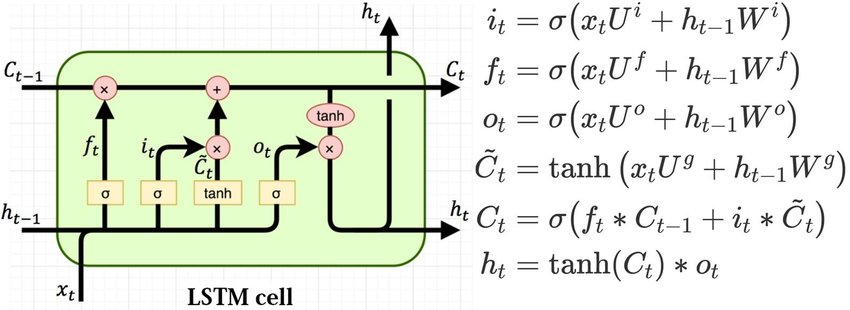
\includegraphics{Plots/image1.png}
\caption{Structure of LSTM and equations describing the gates}
\end{figure}

\begin{enumerate}
\def\labelenumi{\arabic{enumi}.}
\tightlist
\item
  \emph{Cell} \emph{State}: The cell state is the long-term memory of
  the LSTM. It runs straight through the entire sequence, and the LSTM
  can selectively add or remove information from it using gates. The
  cell state acts as a conveyor belt, allowing information to flow while
  preserving relevant information.
\item
  \emph{Forget} \emph{Gate}: The forget gate determines which
  information from the previous time step shou ld be discarded from the
  cell state. It takes as input the current input and the previous
  hidden state and outputs a value between 0 and 1 for each element of
  the cell state. A value of 0 indicates that the corresponding element
  should be forgotten, while a value of 1 indicates that it should be
  retained.
\item
  \emph{Input} \emph{Gate} and \emph{Output} \emph{Gate}: The input gate
  and output gate control the flow of information into and out of the
  memory cell. The input gate determines which values from the current
  time step should be updated in the cell state, while the output gate
  controls which values from the cell state should be used to compute
  the output of the LSTM.
\end{enumerate}

Using these gates and memory cells, an LSTM model can effectively
capture long-term dependencies in time series data. During training, the
model learns the optimal parameters for the gates and the memory cells
by minimising a loss function that measures the model's performance in
predicting the target values.

In the context of univariate time series analysis, an LSTM model takes
the past values of a single variable as input and predicts the future
values of that variable. It can be trained on a historical sequence of
data and then used to forecast future values based on the learned
patterns and dependencies in the data.

Overall, LSTM models have proven to be powerful tools for time series
analysis, enabling accurate predictions and capturing complex temporal
patterns in univariate data.

\hypertarget{prophet}{%
\subsubsection{Prophet}\label{prophet}}

Prophet is a forecasting model developed by Facebook's Core Data Science
team. It is designed to handle time series data with various components
such as trends, seasonality, and holiday effects. Prophet utilises an
additive model that decomposes the time series into its constituent
parts and models them separately.

The Prophet model incorporates the following components:

\begin{enumerate}
\def\labelenumi{\arabic{enumi}.}
\item
  \emph{Trend}: Prophet captures both short-term and long-term trends in
  the data. It employs a piecewise linear or logistic growth curve to
  model non-linear changes in the trend.

  \begin{itemize}
  \item
    Linear - A linear trend refers to a pattern in the data where the
    values increase or decrease steadily and consistently over time or
    across a range of observations.
  \item
    Logistic - A logistic trend refers to a pattern in the data where
    the values initially increase or decrease rapidly, but eventually
    level off or reach a plateau. It is commonly observed in situations
    where there are limiting factors or constraints on the growth or
    decline of a variable. The logistic trend is characterised by an
    initial exponential-like growth or decline, followed by a gradual
    flattening of the curve.
  \end{itemize}
\item
  \emph{Seasonality}: Prophet accounts for recurring patterns in the
  data, such as weekly, monthly, or yearly seasonality. It uses Fourier
  series to model these seasonal components.
\item
  \emph{Holidays}: Prophet incorporates the impact of holidays or
  important events that may affect the time series. It allows users to
  provide a custom list of holidays or automatically detects holidays
  based on country-specific datasets.
\item
  \emph{Error}: Prophet assumes that the observed time series is a
  combination of trend, seasonality, and noise. It models the residual
  errors using a non-parametric approach based on historical data.
\end{enumerate}

Equation of the Prophet Model is:

\(Y(t) = g(t) + s(t) + h(t) + e(t)\).

where \(g(t)\): trend, \(s(t)\): seasonality, \(h(t)\): holiday effects,
and \(e(t)\): error term/noise

Prophet offers several advantages for time series forecasting:

\begin{enumerate}
\def\labelenumi{\arabic{enumi}.}
\item
  Flexibility: It can handle time series data with irregular gaps,
  missing values, and outliers.
\item
  Automatic changepoint detection: Prophet automatically detects
  changepoints in the trend, allowing for capturing abrupt changes in
  the time series.
\item
  Intuitive model interpretation: Prophet provides clear and
  interpretable visualisations, including trend, seasonality, and
  holiday effects, enabling users to understand the underlying patterns.
\item
  Scalability: Prophet can handle large-scale time series datasets
  efficiently and can be parallelized for faster computation.
\end{enumerate}

To use the Prophet model, users need to provide a historical time series
dataset with a timestamp column and a corresponding value column.
Prophet then fits the model to the data, estimates the model parameters,
and provides forecasts for future time points.

\hypertarget{tsmc}{%
\section{TSMC}\label{tsmc}}

TSMC (Taiwan Semiconductor Manufacturing Company) is a global leader in
semiconductor manufacturing and the world's largest dedicated
independent semiconductor foundry. Established in 1987, TSMC has played
a pivotal role in shaping the technology landscape and driving
innovation in the semiconductor industry.

As a foundry, TSMC specialises in the fabrication of advanced
semiconductor products for a wide range of applications, including
consumer electronics, automotive, telecommunications, and industrial
devices. The company's cutting-edge manufacturing processes enable the
production of high-performance chips, delivering enhanced computational
power, energy efficiency, and miniaturisation.

Most of the leading fabless semiconductor companies such as AMD, Apple,
ARM, Broadcom, Marvell, MediaTek, Qualcomm, and Nvidia, are customers of
TSMC, as are emerging companies such as Allwinner Technology, HiSilicon,
Spectra7, and UNISOC.

\hypertarget{data-and-insights}{%
\subsection{Data and Insights}\label{data-and-insights}}

All datasets utilised in this project were sourced exclusively from the
official website of TSMC, ensuring data authenticity and reliability.
The dataset employed for time series analysis comprises monthly revenue
data spanning from January 1999 to April 2023. The revenue values are
reported in units of 1 billion NTD (New Taiwanese Dollar).

\begin{figure}
\centering
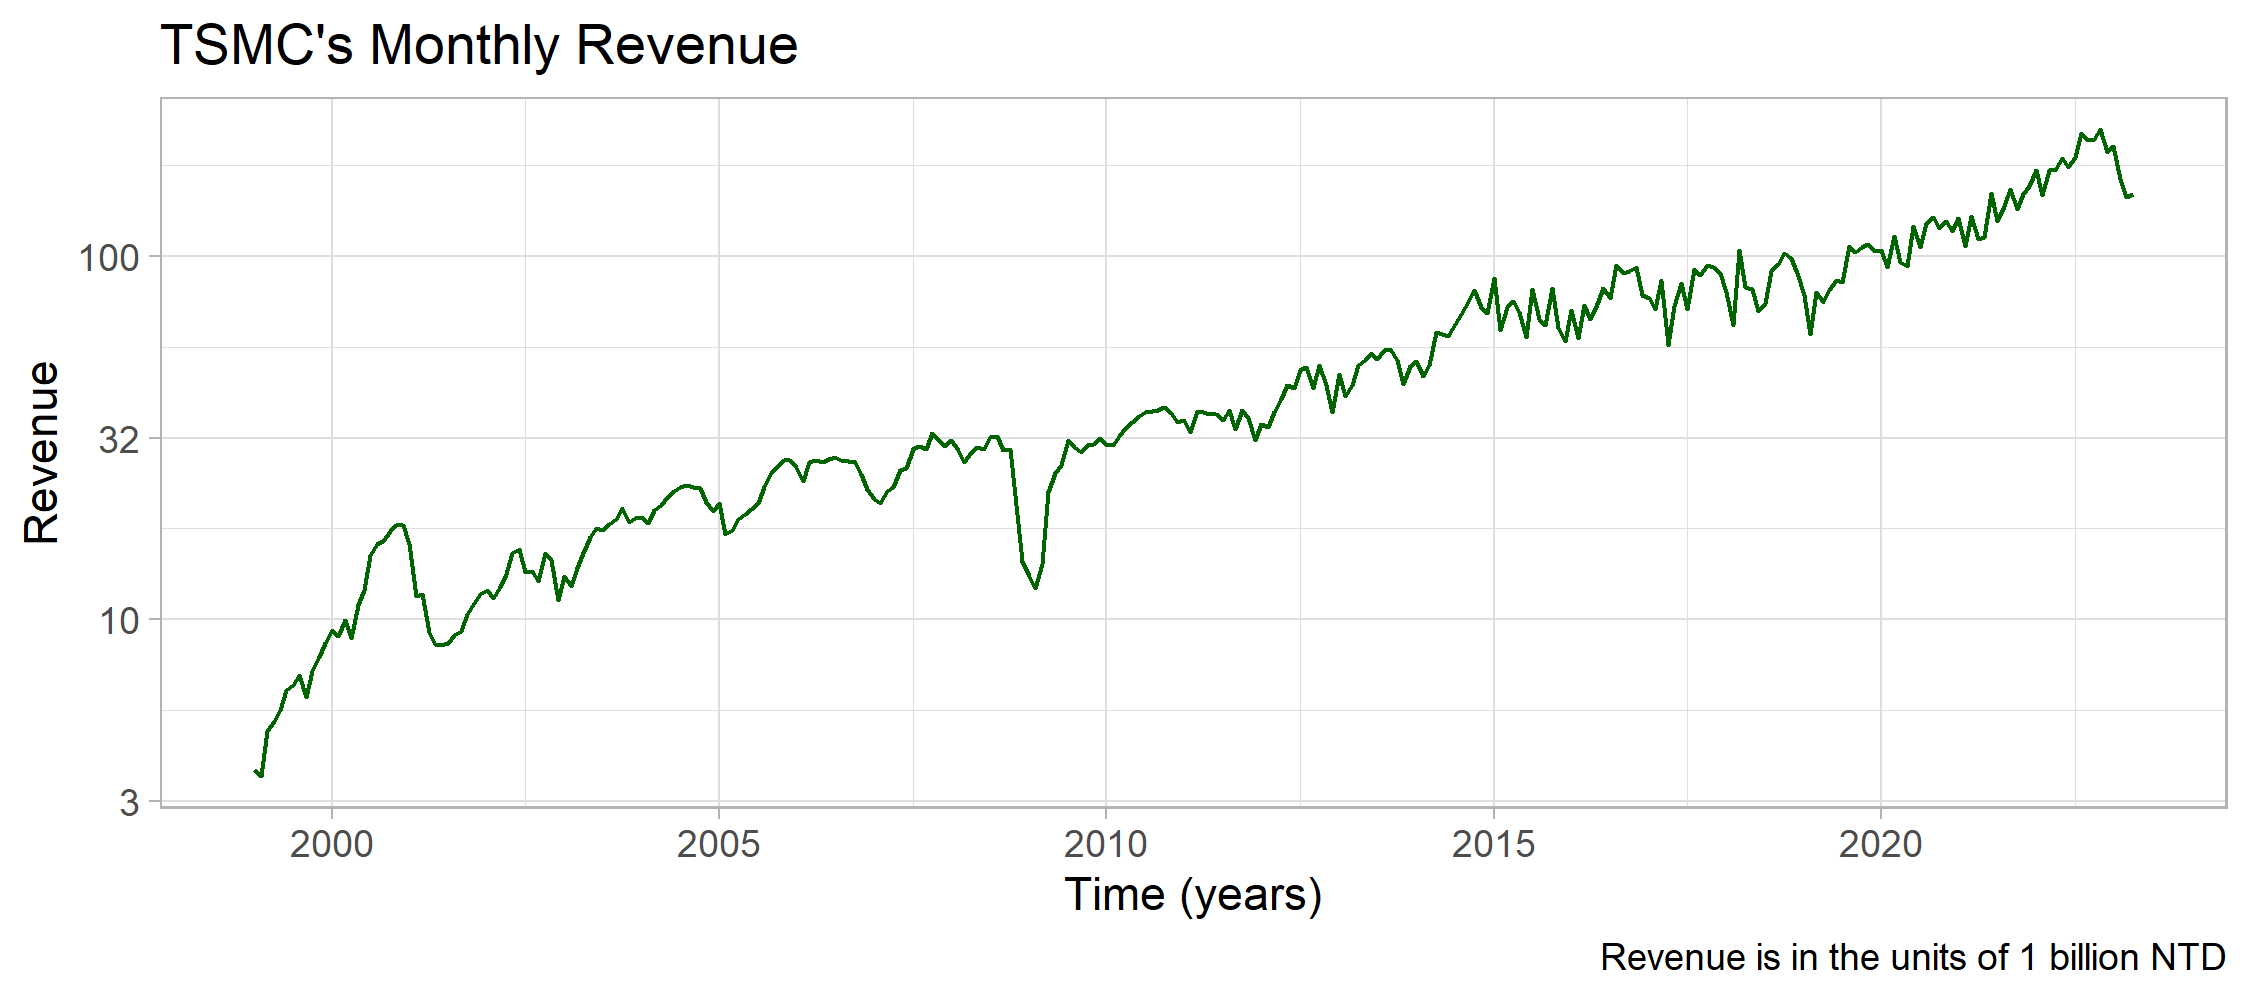
\includegraphics{Plots/RevenuePlot.png}
\caption{Monthly revenue of TSMC from January 1999 to April 2023
represented on a log scale.}
\end{figure}

\begin{figure}
\centering
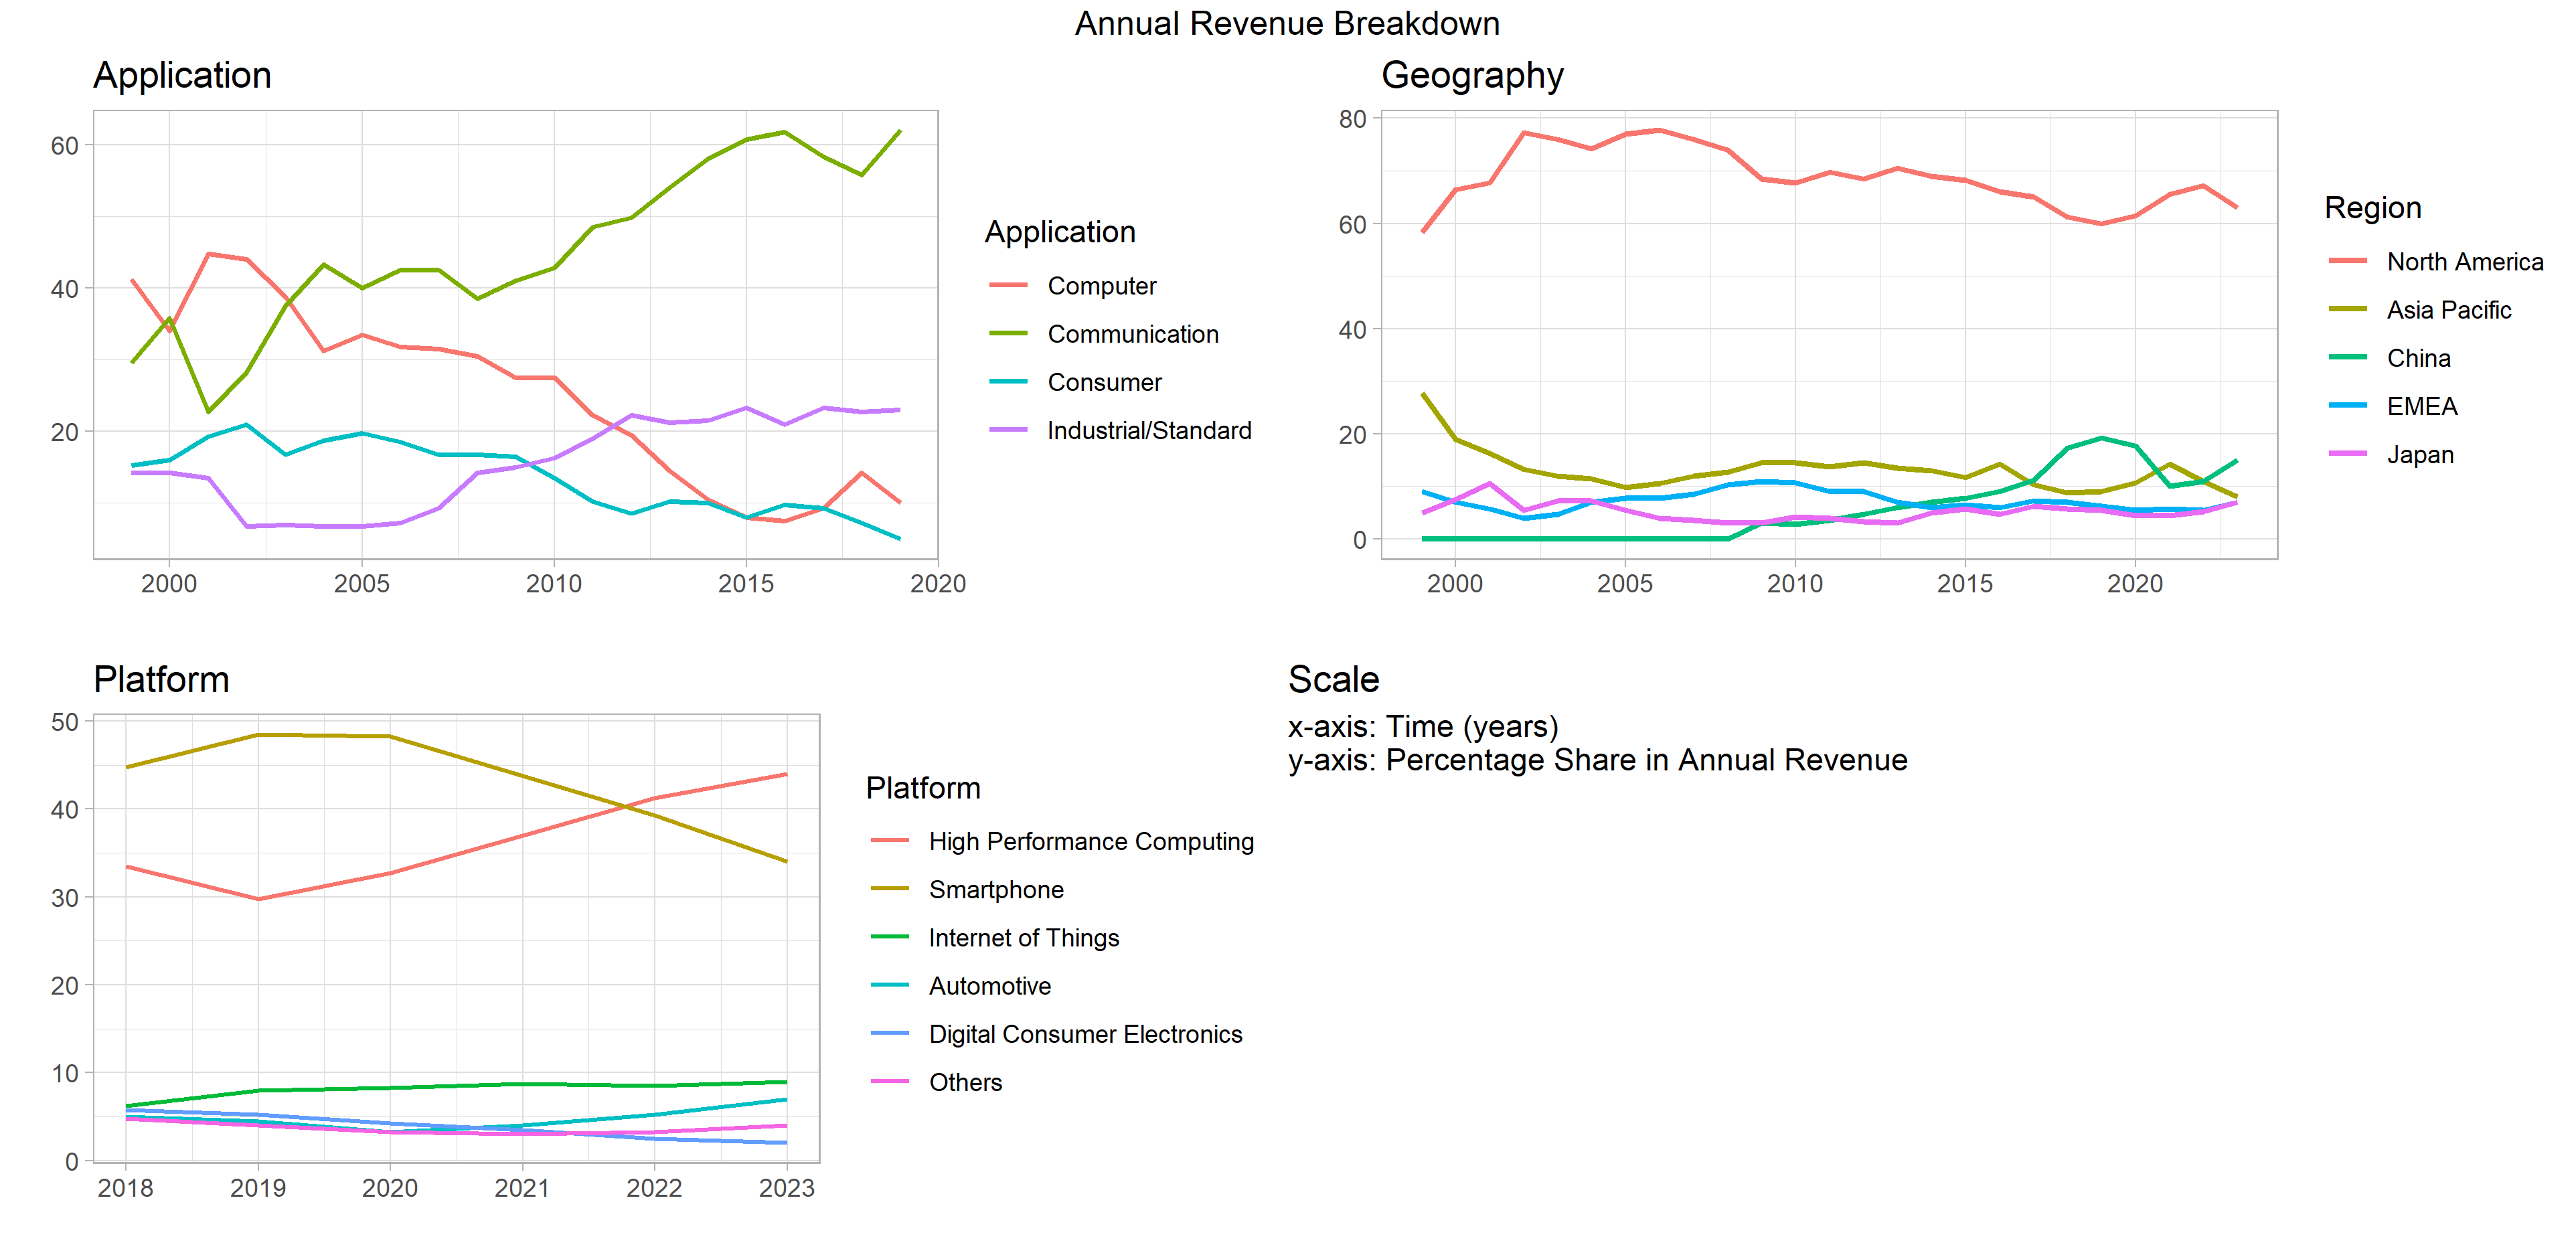
\includegraphics{Plots/RevenueBreakdown.png}
\caption{Breakdown of the annual revenue of TSMC by application,
geography and platform.}
\end{figure}

\hypertarget{analysis-and-results}{%
\section{Analysis and Results}\label{analysis-and-results}}

Initially, we extract valuable insights from the plotted data. As
depicted in Figure 3, the monthly revenue exhibits an approximately
linear trend when visualised on a logarithmic scale. This observation
leads us to consider employing models that assume a linear trend in the
data, such as ARIMA, Holt Winters, and FB Prophet. For the purpose of
analysis, we adopt a logarithmic transformation using a base of 10.

\hypertarget{sarima}{%
\subsection{SARIMA}\label{sarima}}

Let us denote our original revenue time series by \(R_{t}\) . We have
292 data points from January 1999 to April 2023 hence
\(t \in \left\{ 1,\ 2,\ .\ .\ .\ 292 \right\}\). In order to fit the
SARIMA model we first need to make the time series stationary. As
mentioned earlier we take log of \(R_{t}\) to get
\(Y_{t} = \log_{10}(R_{t})\). We apply a first order differencing to
\(Y_{t}\) to get \(Z_{t} = Y_{t} - Y_{t - 1}\).

\begin{figure}
\centering
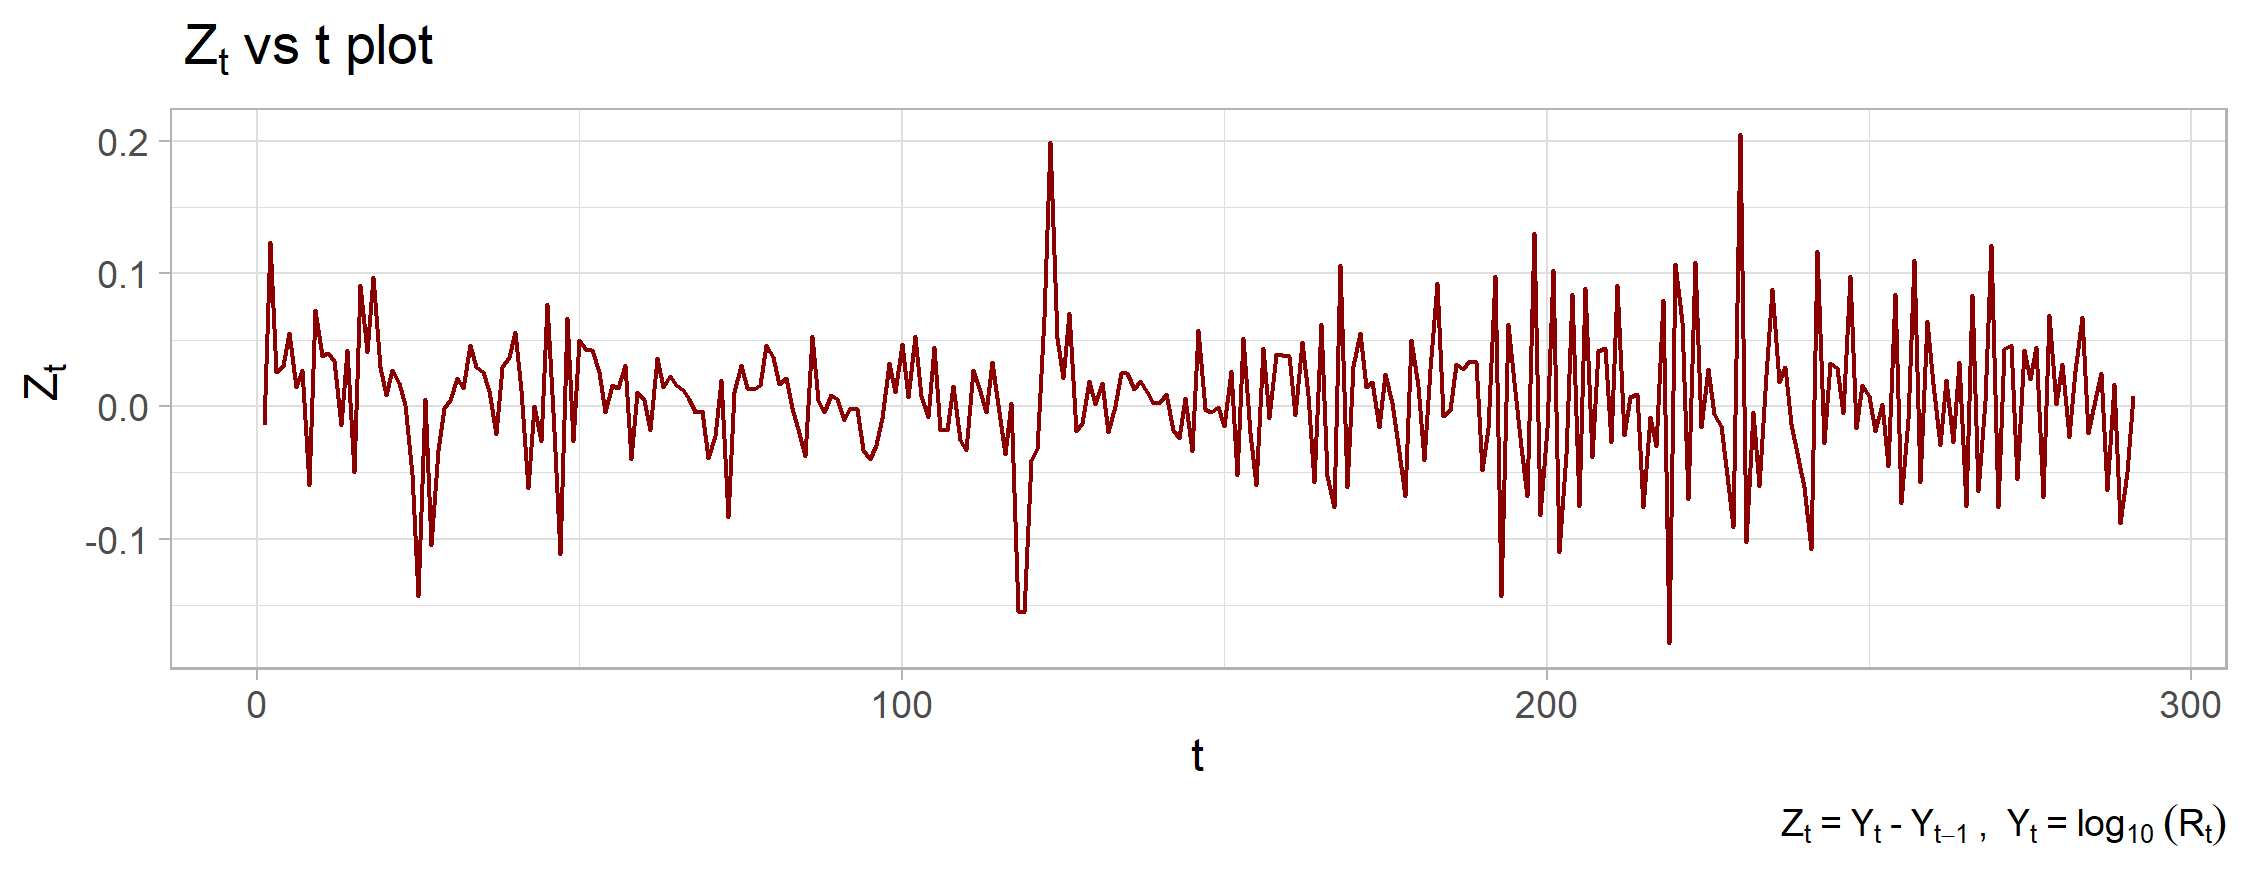
\includegraphics{Plots/Ztplot.png}
\caption{Plot showing the differenced timeseries.}
\end{figure}

We perform the ADF test on \(Z_{t}\) with lag order 24 to check if we
have acheived stationarity or not. The p-value returned is 0.01
therefore we reject the null hypothesis of non-stationariy. Hence in the
SARIMA model the order of differencing \(d = 1\) and the order of
seasonal differencing \(D=0\). Now to find the value of
\(p, P, Q, \text{and } q\) we look at the ACF and PACF plots. The PACF
plot shows the direct correlation between \(Z_{t}\) and \(Z_{t - k}\)
where k is the number of lags. The largest \(k\) for which the PACF
value is significantly different from zero gives a good measure for the
value of \(p\). The ACF plot shows the direct correlation for
\(Z_{t}\)and \(Z_{t - k}\). The largest \(k\) for which the ACF value is
significantly different from zero gives a good measure of \(q\).
\(P,\text{ and } Q\)are also found similarly. Since some correlation
might arise from random chance and may not reflect the underlying data
generation process we have to consider multiple values for \(p\) and
\(q\) and then select the best. AICc value is used to choose the best
model.

\begin{figure}
\centering
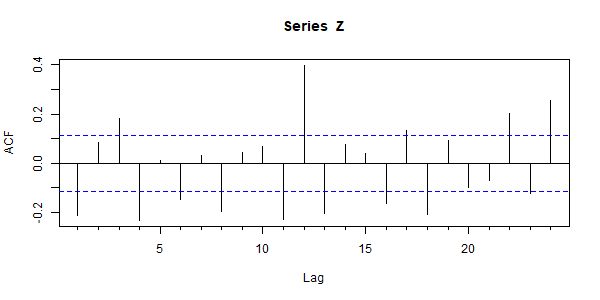
\includegraphics{Plots/acfZ.png}
\caption{Plot of the auto correlation function of the differenced
timeseries as a function of lags}
\end{figure}

\begin{figure}
\centering
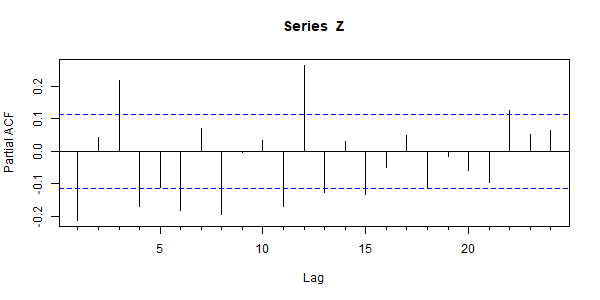
\includegraphics{Plots/pacfZ.png}
\caption{Plot of the partial autocorrelation function of the differenced
timeseries as a function of lags.}
\end{figure}

The spike in the PACF plot at lag = 12 suggests that the seasonal period
\(m\) is 12. Using the plots we guess that \(p\  \in \ \{ 1,\ 3,\ 4\}\)
, \(q\  \in \{ 1,\ 3,\ 4\}\), \(D \in \{ 0\}\), \(P \in \{ 1\}\),
\(Q \in \{ 0,1,\ 2\}\). Now we take all possible combinations of
\(p, q,\) and \(Q\) and calculate the AICc value for each of them.

The values of \(p, q,\) and \(Q\) which minimise AICc are 4, 1, and 2
respectively. Hence the SARIMA model that we get is
\(SARIMA(4,1,1)(1,0,2)[12]\).

\begin{longtable}[]{@{}
  >{\raggedright\arraybackslash}p{(\columnwidth - 16\tabcolsep) * \real{0.1111}}
  >{\raggedright\arraybackslash}p{(\columnwidth - 16\tabcolsep) * \real{0.1111}}
  >{\raggedright\arraybackslash}p{(\columnwidth - 16\tabcolsep) * \real{0.1111}}
  >{\raggedright\arraybackslash}p{(\columnwidth - 16\tabcolsep) * \real{0.1111}}
  >{\raggedright\arraybackslash}p{(\columnwidth - 16\tabcolsep) * \real{0.1111}}
  >{\raggedright\arraybackslash}p{(\columnwidth - 16\tabcolsep) * \real{0.1111}}
  >{\raggedright\arraybackslash}p{(\columnwidth - 16\tabcolsep) * \real{0.1111}}
  >{\raggedright\arraybackslash}p{(\columnwidth - 16\tabcolsep) * \real{0.1111}}
  >{\raggedright\arraybackslash}p{(\columnwidth - 16\tabcolsep) * \real{0.1111}}@{}}
\caption{Parameters of the SARIMA model.}\tabularnewline
\toprule\noalign{}
\begin{minipage}[b]{\linewidth}\raggedright
\end{minipage} & \begin{minipage}[b]{\linewidth}\raggedright
\(\phi_1\)
\end{minipage} & \begin{minipage}[b]{\linewidth}\raggedright
\(\phi_2\)
\end{minipage} & \begin{minipage}[b]{\linewidth}\raggedright
\(\phi_3\)
\end{minipage} & \begin{minipage}[b]{\linewidth}\raggedright
\(\phi_4\)
\end{minipage} & \begin{minipage}[b]{\linewidth}\raggedright
\(\theta_1\)
\end{minipage} & \begin{minipage}[b]{\linewidth}\raggedright
\(\phi_{12}\)
\end{minipage} & \begin{minipage}[b]{\linewidth}\raggedright
\(\theta_{12}\)
\end{minipage} & \begin{minipage}[b]{\linewidth}\raggedright
\(\theta_{24}\)
\end{minipage} \\
\midrule\noalign{}
\endfirsthead
\toprule\noalign{}
\begin{minipage}[b]{\linewidth}\raggedright
\end{minipage} & \begin{minipage}[b]{\linewidth}\raggedright
\(\phi_1\)
\end{minipage} & \begin{minipage}[b]{\linewidth}\raggedright
\(\phi_2\)
\end{minipage} & \begin{minipage}[b]{\linewidth}\raggedright
\(\phi_3\)
\end{minipage} & \begin{minipage}[b]{\linewidth}\raggedright
\(\phi_4\)
\end{minipage} & \begin{minipage}[b]{\linewidth}\raggedright
\(\theta_1\)
\end{minipage} & \begin{minipage}[b]{\linewidth}\raggedright
\(\phi_{12}\)
\end{minipage} & \begin{minipage}[b]{\linewidth}\raggedright
\(\theta_{12}\)
\end{minipage} & \begin{minipage}[b]{\linewidth}\raggedright
\(\theta_{24}\)
\end{minipage} \\
\midrule\noalign{}
\endhead
\bottomrule\noalign{}
\endlastfoot
Value & 0.8218 & 0.1028 & 0.2128 & -0.3186 & -0.9289 & 0.9892 & -0.7017
& -0.2032 \\
S.D. & 0.0672 & 0.0749 & 0.0746 & 0.0571 & 0.0387 & 0.0216 & 0.0814 &
0.0783 \\
\end{longtable}

In order to get the final model equation we need to find out which
coefficients are statistically different from 0. If the value of the
coefficients is within two standard deviations of 0 then we say that
that coefficient is statistically equivalent to 0 hence we will not
include it in the model equation. We find that ar2 should not be
included.

\(Z_{t} = 0.822\ Z_{t - 1} + 0.213\ Z_{t - 3} - 0.319{\ Z}_{t - 4} - 0.929\ \varepsilon_{t - 1} + 0.989\ Z_{t - 12} - 0.702\ \varepsilon_{t - 12} - 0.203\ \varepsilon_{t - 24}\)

\(Y_{t} = Z_{t} + Y_{t - 1}\)

\begin{figure}
\centering
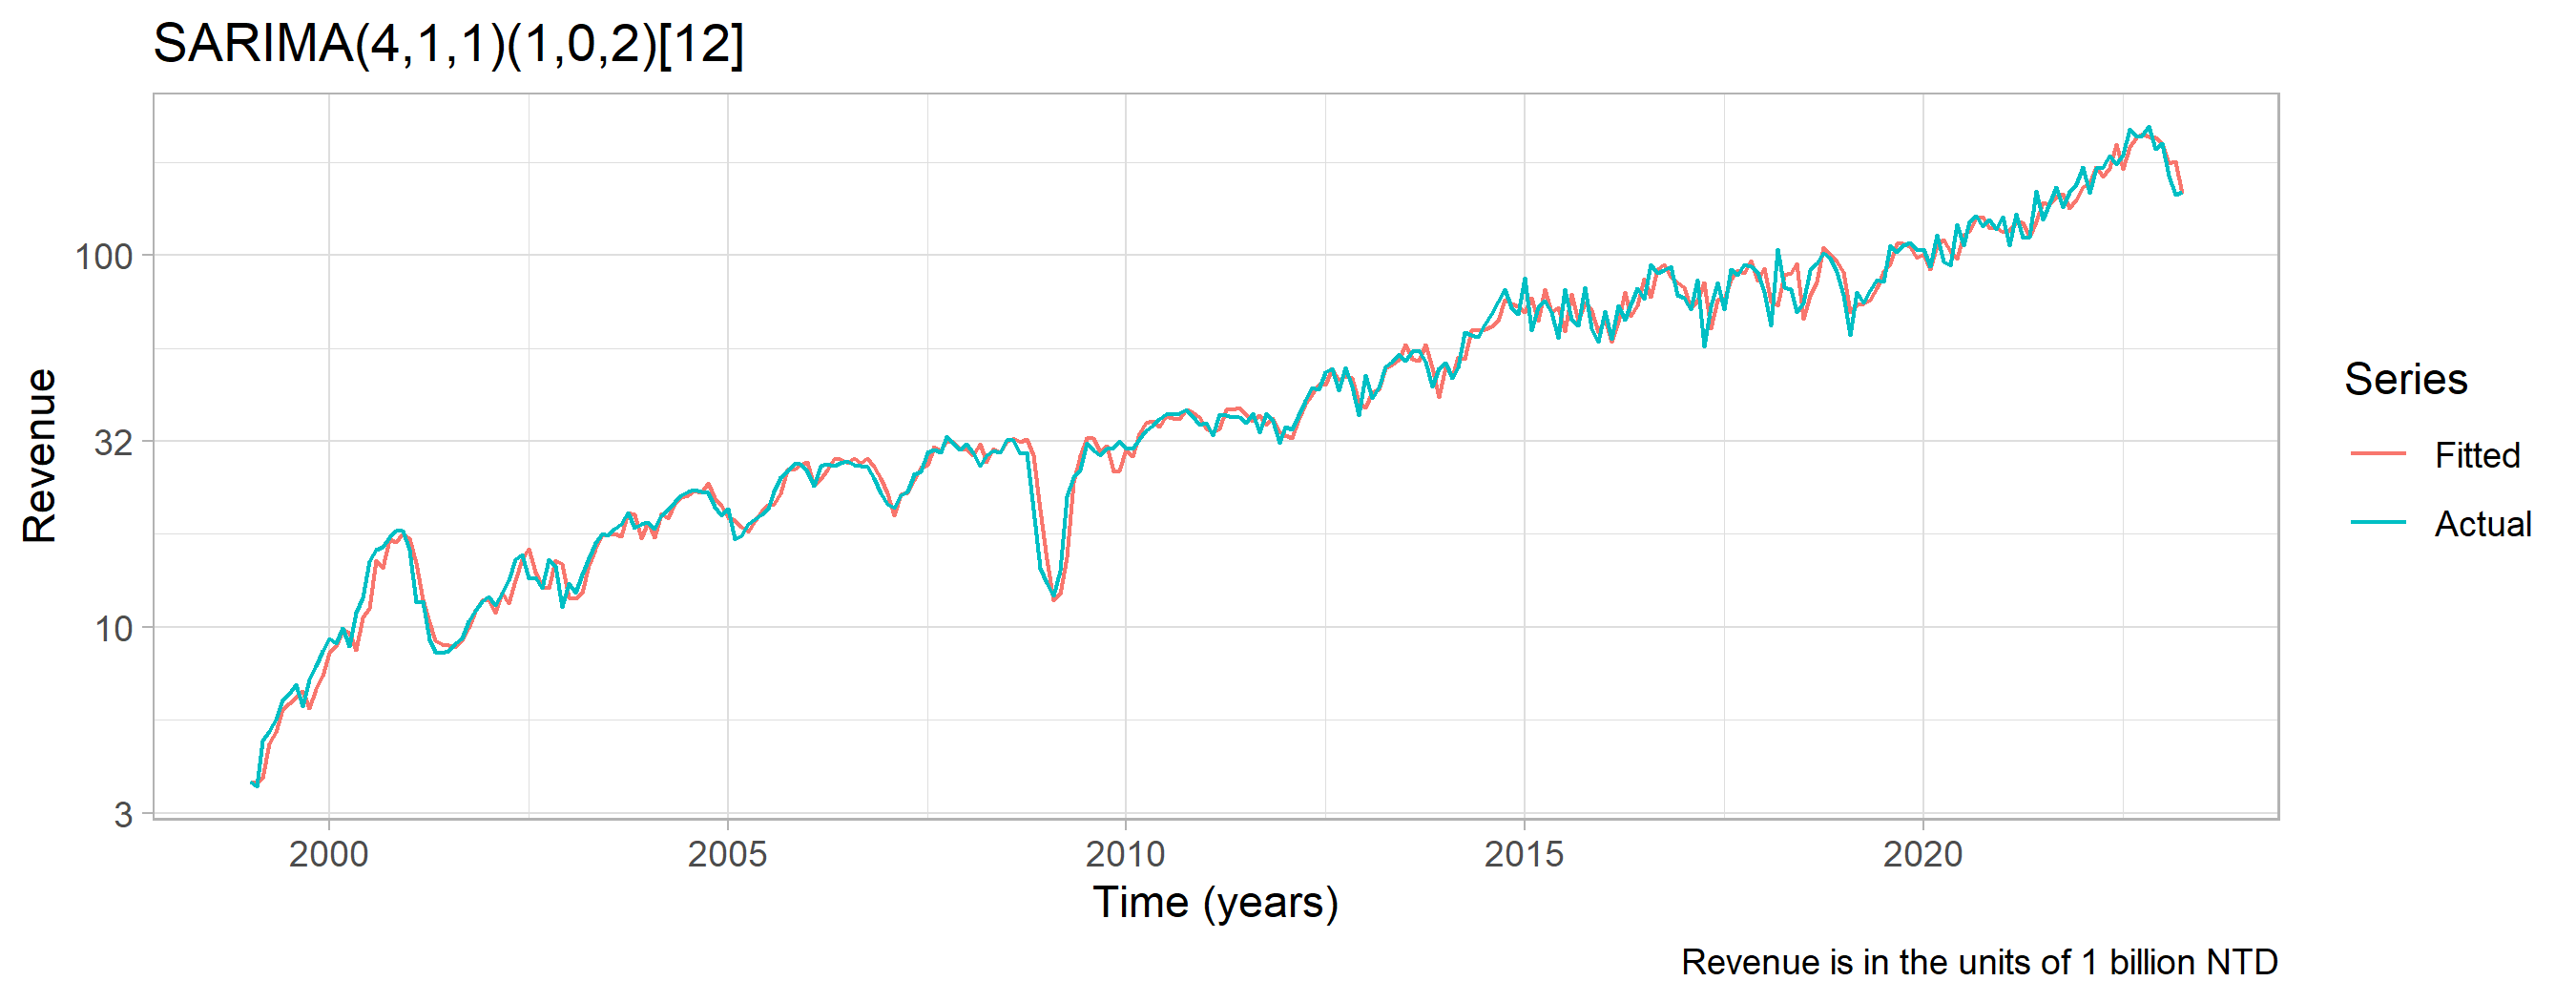
\includegraphics{Plots/fittedarimaplot.png}
\caption{Fitted values of the SARIMA model.}
\end{figure}

If our model is good then the residuals should be IID normal random
variables i.e.~white noise. Ljung-Box test with the number of lags = 24
on our residuals gives us a p-value of 0.36 which shows that the
residuals are in fact white noise.

\hypertarget{holt-winters}{%
\subsection{Holt-Winters}\label{holt-winters}}

Following the same procedure as in the SARIMA model we fit our model on
\(Z_{t}\). We use the same seasonal period = 12. The smoothing parameter
\(\alpha,\ \beta,\) and \(\gamma\) are estimated by minimising the mean
squared error.

\(\alpha = 0.0008\), \(\beta = 0.0008\), \(\gamma = 0.0485\).

The initial values are calculated as:\\
\(l_{12} = mean(Z_{1}, Z_{13}, \dots) ,\ b_{12} = mean(\frac{Z_{13} - Z_{1}}{12}, \frac{Z_{14} - Z_{2}}{12} ,\dots) , s_{i} = Z_{i} - l_{12} ,\forall \ i \ \in \ \{1,\ 2, \dots 12\}\)

\(\forall\ t\  > \ 12,\)

\(l_{t} = \alpha(Z_{t} - s_{t - 12}) + (1 - \alpha)(l_{t - 1} - b_{t - 1})\)

\(b_{t} = \beta(l_{t} - l_{t - 1}) + (1 - \beta)b_{t - 1}\)

\(s_{t} = \gamma(Z_{t} - l_{t - 1} - b_{t - 1}) + (1 - \gamma)s_{t - 12}\)

\(Z_{t} = l_{t - 1} + b_{t - 1} + s_{t - 12}\)

\(Y_{t} = Z_{t} + Y_{t - 1}\)

\begin{longtable}[]{@{}
  >{\raggedright\arraybackslash}p{(\columnwidth - 12\tabcolsep) * \real{0.1515}}
  >{\raggedright\arraybackslash}p{(\columnwidth - 12\tabcolsep) * \real{0.1515}}
  >{\raggedright\arraybackslash}p{(\columnwidth - 12\tabcolsep) * \real{0.1212}}
  >{\raggedright\arraybackslash}p{(\columnwidth - 12\tabcolsep) * \real{0.1212}}
  >{\raggedright\arraybackslash}p{(\columnwidth - 12\tabcolsep) * \real{0.1515}}
  >{\raggedright\arraybackslash}p{(\columnwidth - 12\tabcolsep) * \real{0.1515}}
  >{\raggedright\arraybackslash}p{(\columnwidth - 12\tabcolsep) * \real{0.1515}}@{}}
\caption{Parameters of the Holt-Winters model.}\tabularnewline
\toprule\noalign{}
\endfirsthead
\endhead
\bottomrule\noalign{}
\endlastfoot
\(l_{12}\) & \(b_{12}\) & \(s_1\) & \(s_2\) & \(s_3\) & \(s_4\) &
\(s_5\) \\
0.0111 & -0.003 & 0.0071 & -0.029 & -0.029 & 0.019 & -0.0064 \\
& & & & & & \\
\(s_6\) & \(s_7\) & \(s_8\) & \(s_9\) & \(s_{10}\) & \(s_{11}\) &
\(s_{12}\) \\
0.026 & 0.0061 & 0.014 & 0.019 & -0.0099 & 0.048 & -0.064 \\
\end{longtable}

\begin{figure}
\centering
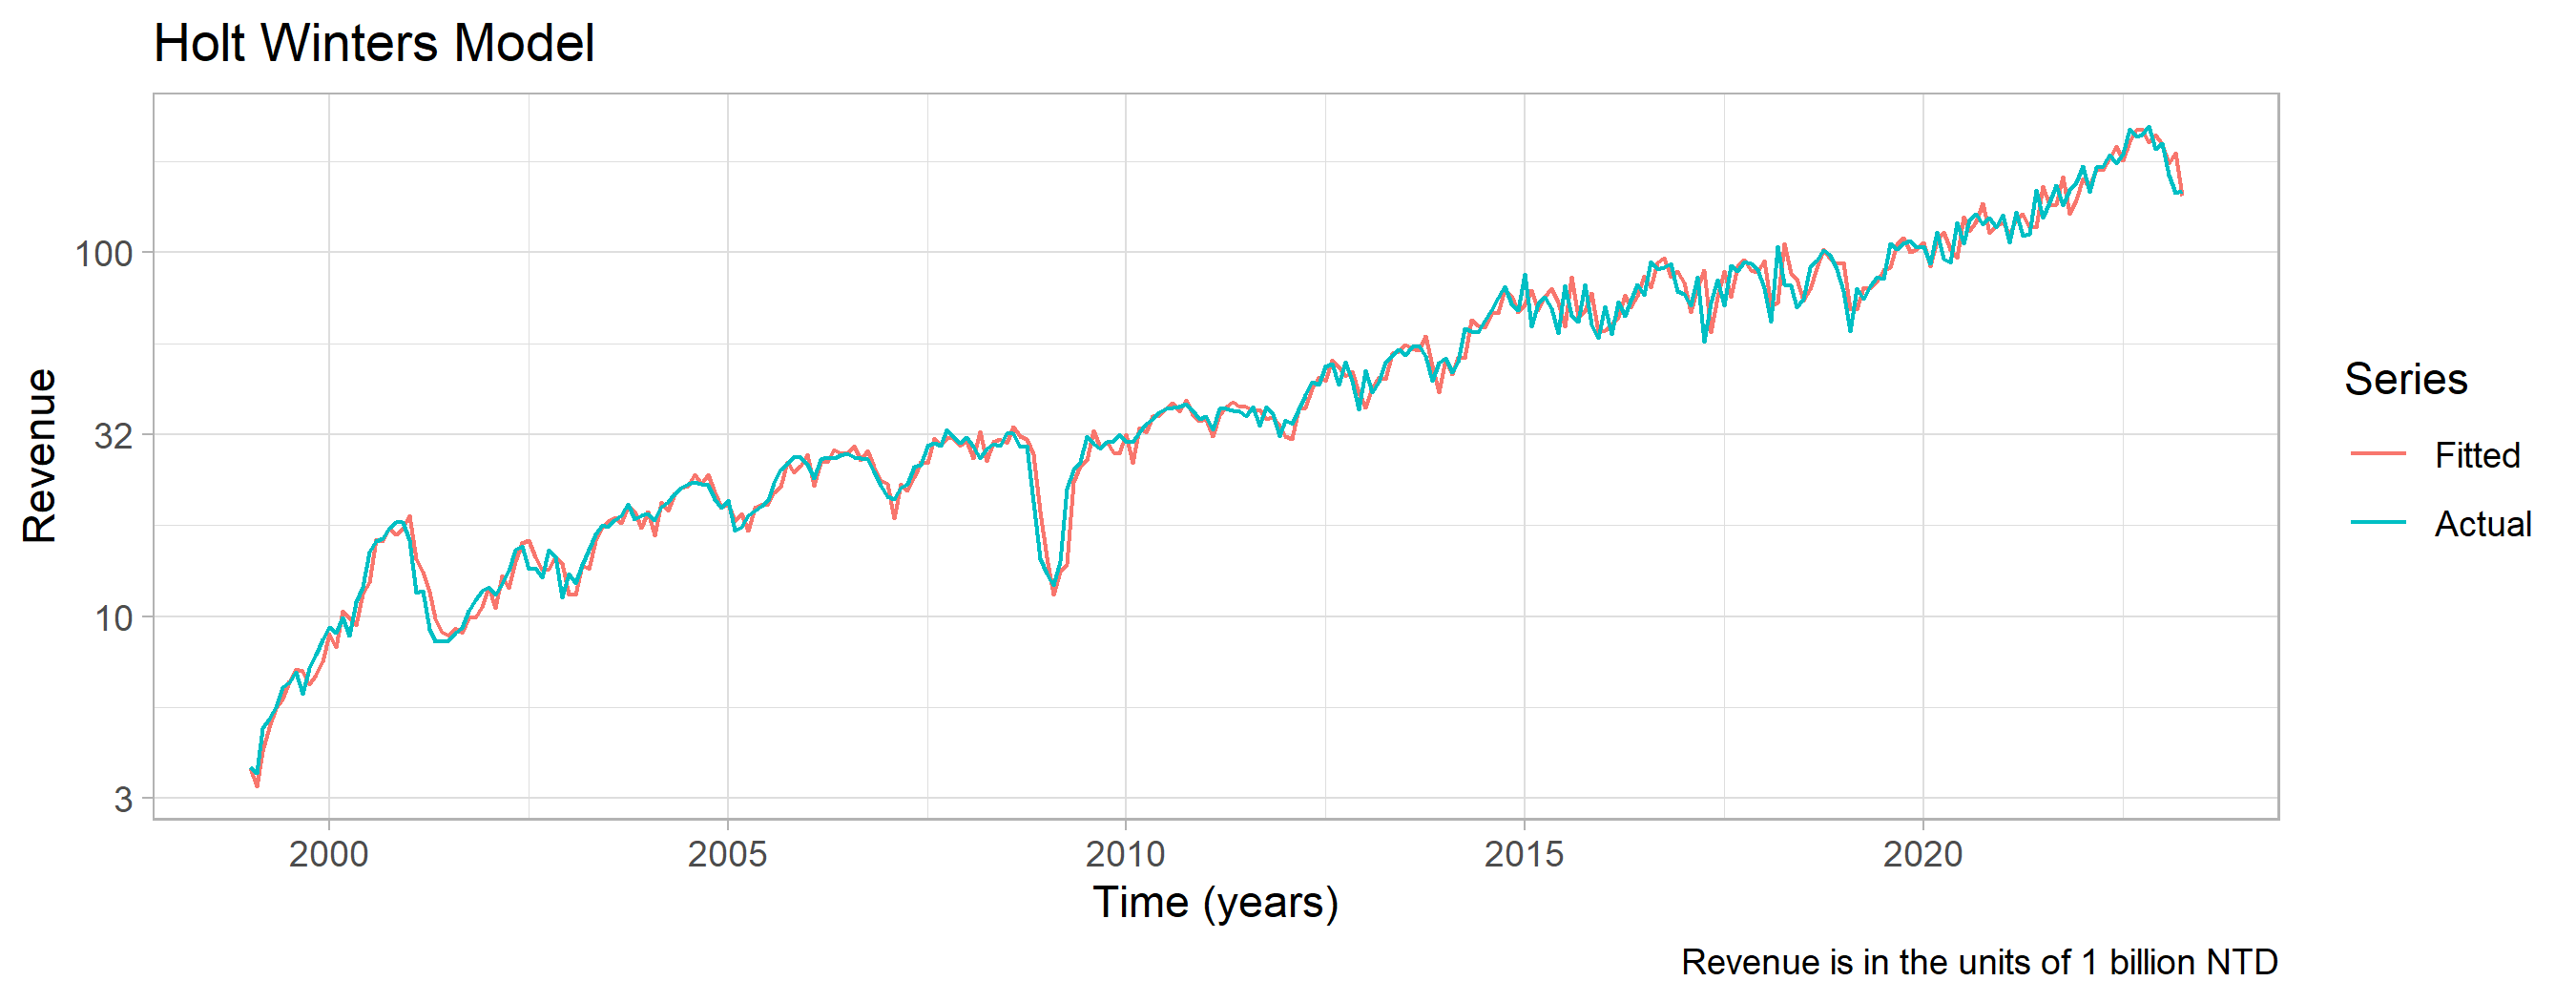
\includegraphics{Plots/fittedhwaddplot.png}
\caption{Fitted values of the Holt-Winters model}
\end{figure}

\hypertarget{prophet-1}{%
\subsection{Prophet}\label{prophet-1}}

The trend component of the Prophet model is modelled as a piecewise
linear function of time. At each changepoint, the trend changes
direction. The trend equation is defined as follows:

\(g(t) = (k + a(t)) \cdot t + d\) where \(g(t)\) : the trend value at
time \(t\), \(k\) : overall growth rate of the trend, \(a(t)\) :
adjustment for each changepoint, and \(d\) : offset parameter, capturing
the overall level of the time series.

Yearly Seasonality Equation :
\[s_{y}(t)\ = \ (A_{j}\ \frac{\cos((2\pi t\ j)}{P})\ + \ B_{j\ }\ \frac{\sin((2\pi t\ j)}{P})\ \]

where \(s_y(t)\) represent the yearly seasonality values at time \(t\).

\(A_{j},\ B_{j}\) are the respective coefficients for the seasonal
components.

\(P\) is the user-defined period for the yearly seasonality (e.g.365.25
for daily data).

The final forecasted value is obtained by summing the trend,
seasonality, and holiday components:

\(y(t) = \ g(t) + s_{y}(t) + h(t) + \ \varepsilon\) where: \(y(t)\) is
the forecasted value at time t and \(\varepsilon\) is the error term
accounting for noise and variability in the time series.

The model is fitted on \(Z_{t}\) with growth set to `linear' and
seasonality mode set to additive.

\begin{figure}
\centering
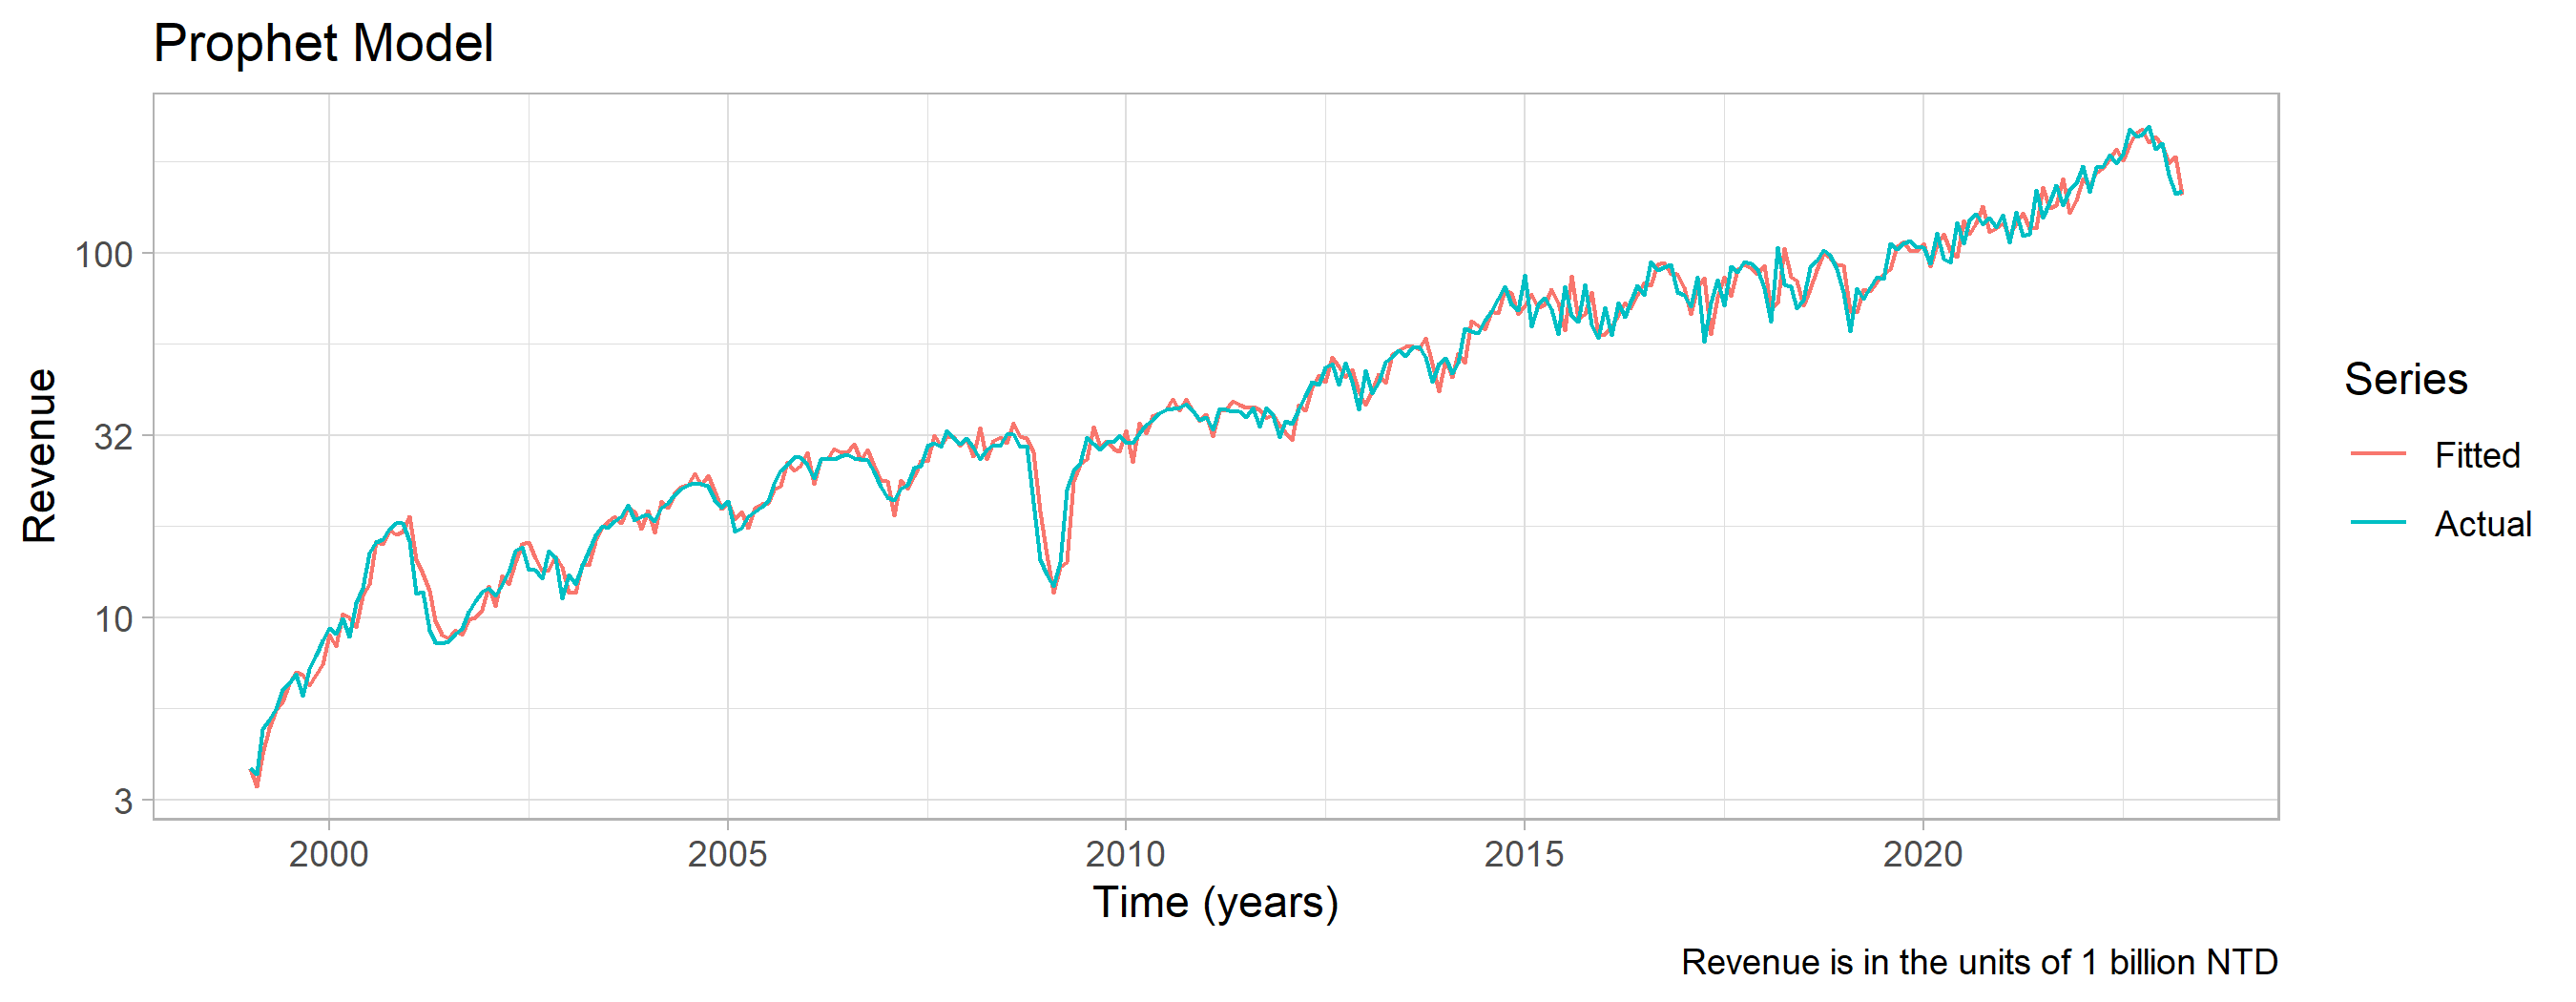
\includegraphics{Plots/fittedprophetplot.png}
\caption{Fitted values for the prophet model.}
\end{figure}

\hypertarget{cross-validation-1}{%
\subsection{Cross Validation}\label{cross-validation-1}}

The objective of our study is to identify the most effective model for
predicting revenue for the upcoming quarter, specifically targeting a
3-month forecasting horizon. To evaluate the performance of the models,
we have adopted the rolling forecast origin cross-validation technique.
This technique involves a systematic process of training and testing the
models using sequential time periods.The methodology can be summarized
as follows:

\begin{figure}
\centering
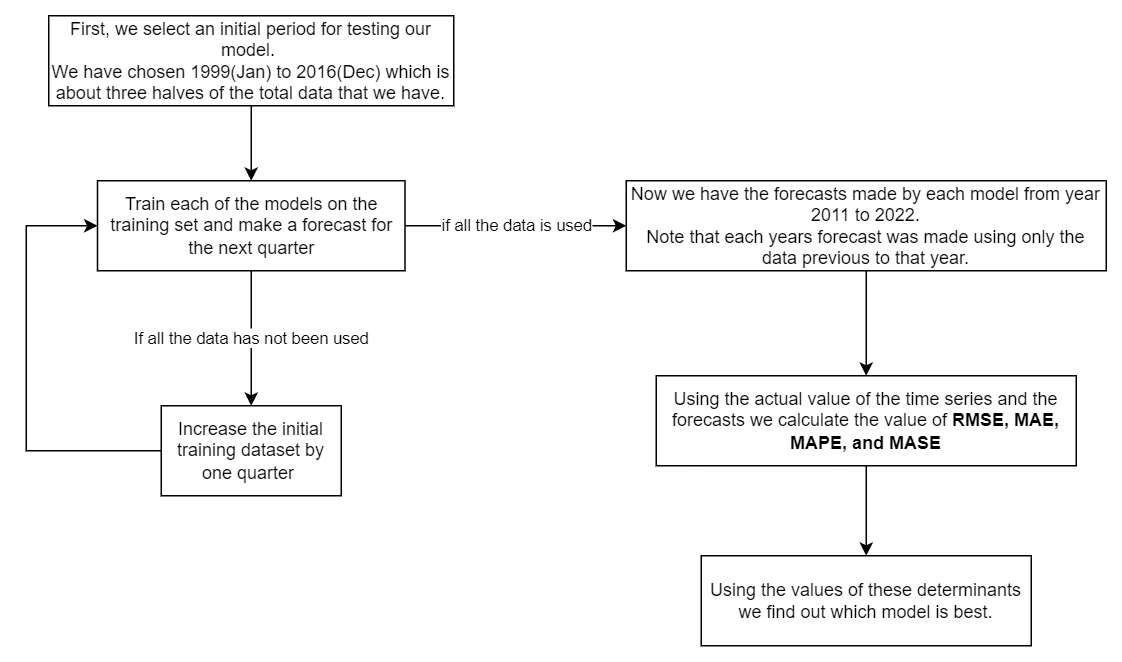
\includegraphics{Plots/crossvalidationflowchart.png}
\caption{Flowchart showing the methodology for cross validation.}
\end{figure}

\begin{figure}
\centering
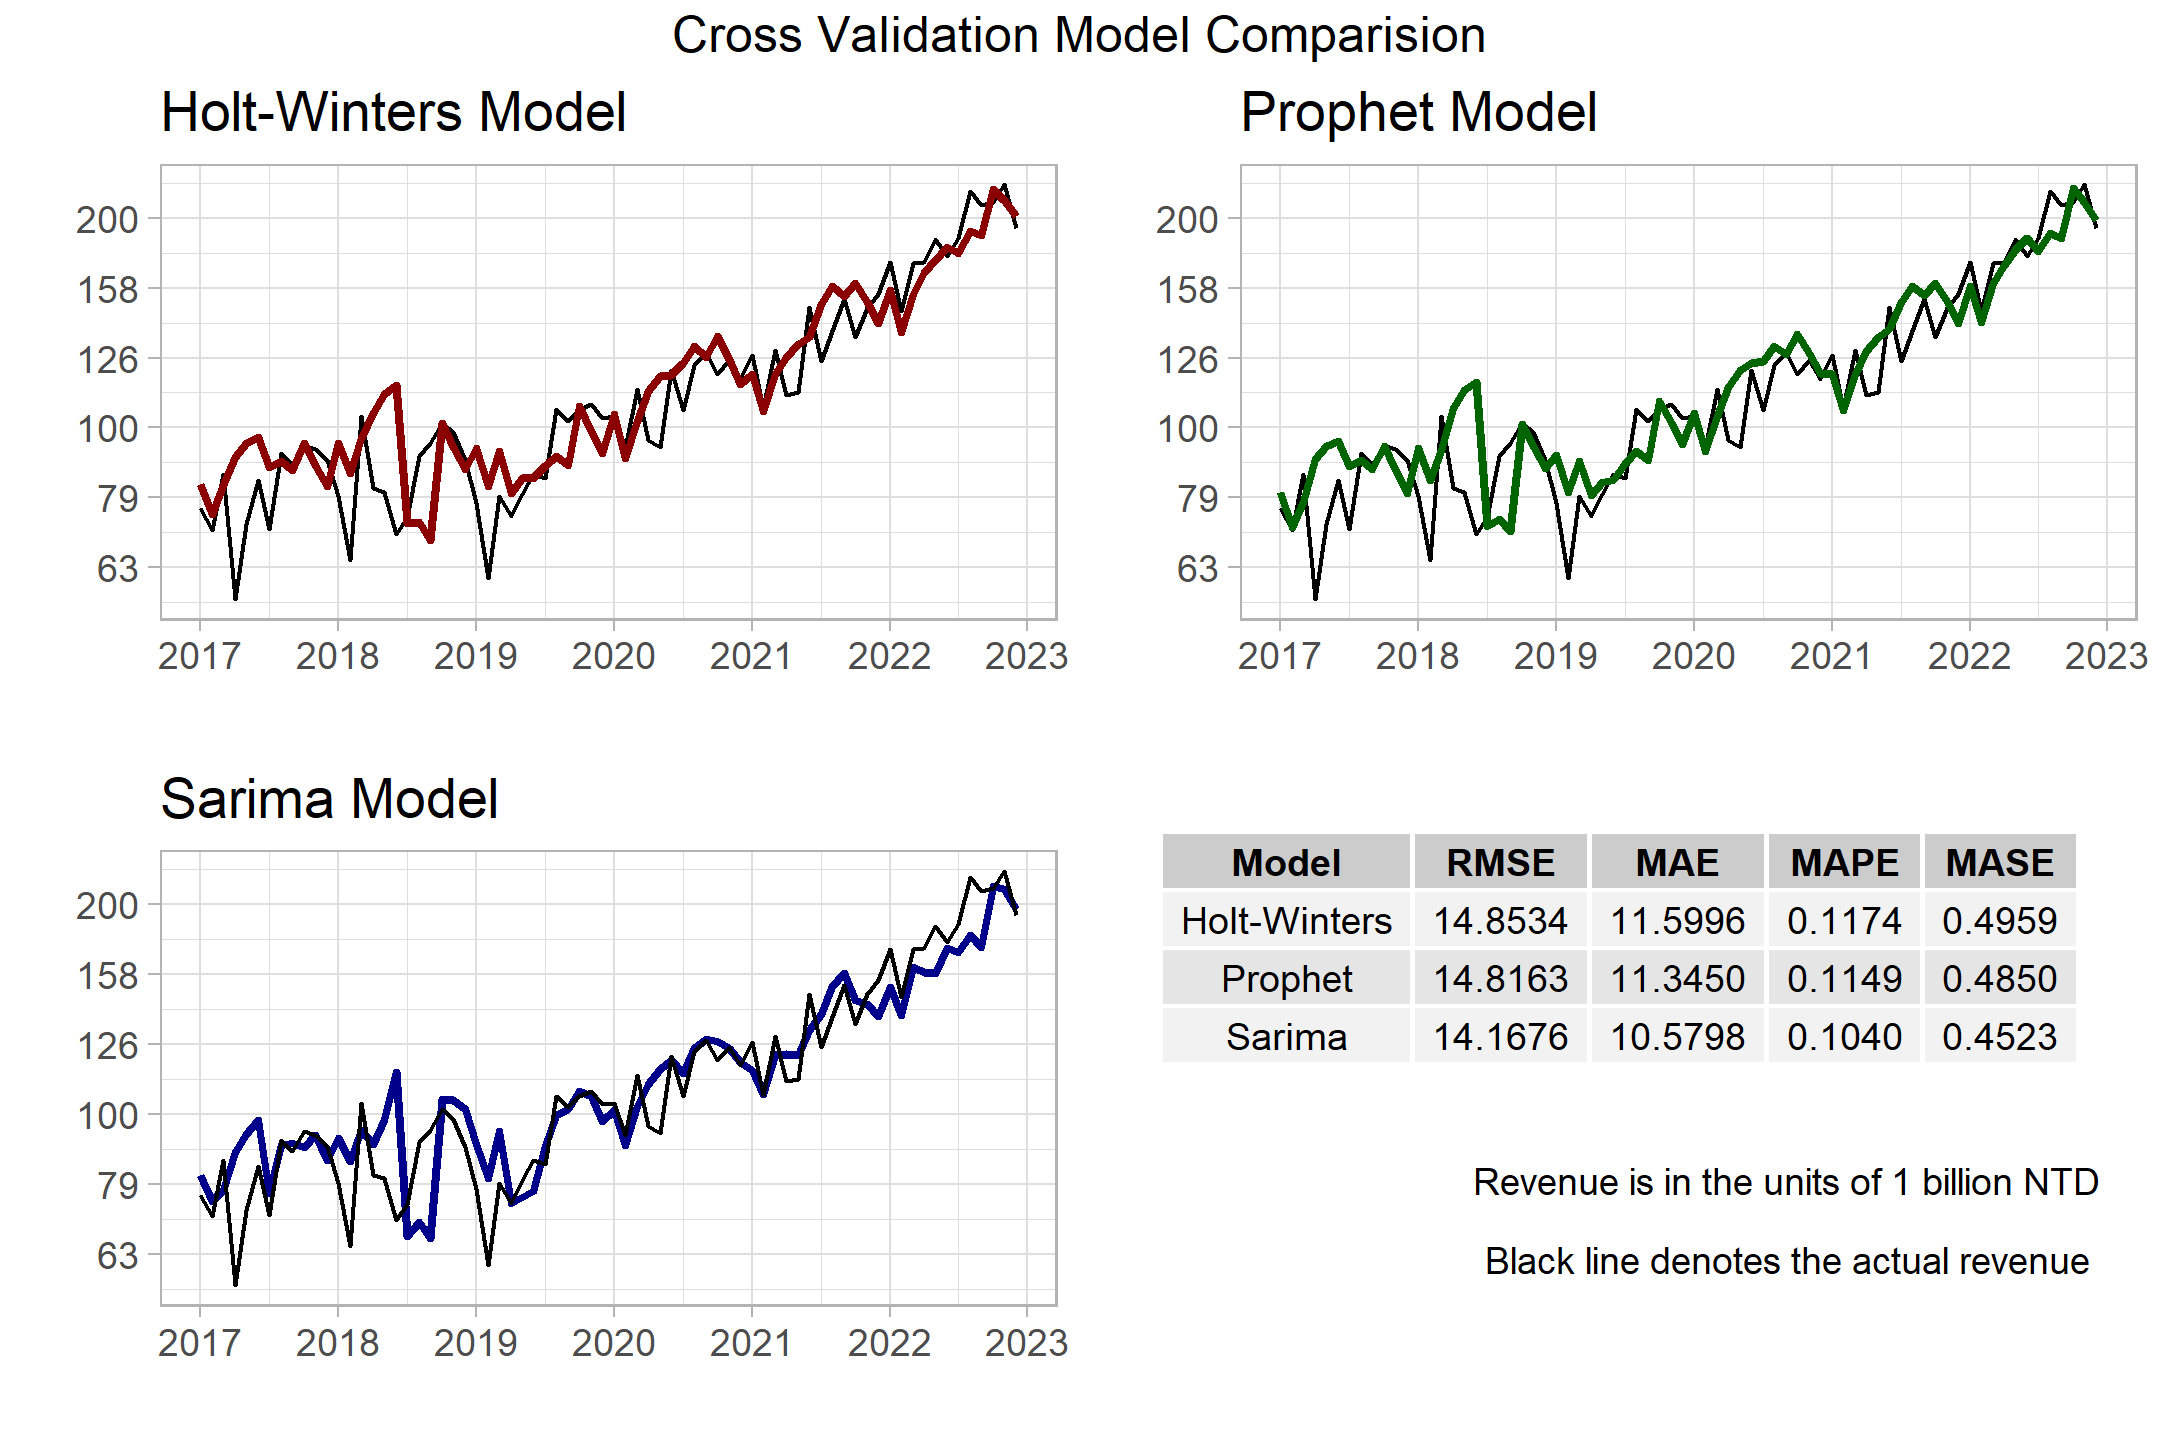
\includegraphics{Plots/CrossValidation.png}
\caption{Plots showing the results of cross validation.}
\end{figure}

\newpage

\hypertarget{conclusion}{%
\section{Conclusion}\label{conclusion}}

Based on the analysis and evaluation of all four determinants, it is
evident that the Prophet model does not outperform the other two models,
namely Holt-Winters and SARIMA. However, it is important to acknowledge
that this study is limited to a specific context, focusing on predicting
the future monthly revenue of TSMC for a 3-month period.

It should be recognized that the performance of the Prophet model may
vary depending on the particular time series under analysis and the
forecasting period considered. Different datasets and forecasting
objectives might yield different results. Therefore, the findings of
this study cannot be generalised to all scenarios and must be
interpreted within the scope of this specific investigation. Further
research and experimentation are necessary to explore the performance of
different models across diverse datasets and forecast scenarios.

Considering the specific case of predicting the future monthly revenue
of TSMC for a 3-month period, the SARIMA model emerges as the superior
choice compared to both Holt-Winters and the Prophet model. The SARIMA
model demonstrated better accuracy and reliability in forecasting
revenue for the given timeframe.

Finally we make the prediction for the next quarter using the Sarima
model

\begin{longtable}[]{@{}lll@{}}
\caption{Forecast for the next quarter using the SARIMA
model.}\tabularnewline
\toprule\noalign{}
Month-Year & Revenue Point Estimate & 90 \% Confidence Interval \\
\midrule\noalign{}
\endfirsthead
\toprule\noalign{}
Month-Year & Revenue Point Estimate & 90 \% Confidence Interval \\
\midrule\noalign{}
\endhead
\bottomrule\noalign{}
\endlastfoot
May 2023 & 150.5297 & (123.4459, 183.5556) \\
June 2023 & 144.7664 & (110.9622, 188.8689) \\
July 2023 & 155.2020 & (112.5692, 213.9810) \\
\end{longtable}

\emph{*Revenue is in the units of 1 billion NTD}

\hypertarget{references}{%
\section{References}\label{references}}

\(^{[1]}\)\emph{C. L. Karmaker, P. K. Halder and E. Sarker} ``A Study of
Time Series Model for Predicting Jute Yarn Demand: Case Study'' ,Journal
of Industrial Engineering, Volume 2017

\(^{[2]}\)\emph{Jana Fabianová*, Peter Kačmáry, Vieroslav Molnár, and
Peter Michalik} ``Using a Software Tool in Forecasting: a Case Study of
Sales Forecasting Taking into Account Data Uncertainty'' ,DE GRUYTER
OPEN, 2016

\(^{[3]}\)\emph{Serkan ARAS , İpek DEVECİ KOCAKOÇ, Cigdem POLAT
``COMPARATIVE STUDY ON RETAIL SALES FORECASTING BETWEEN SINGLE AND
COMBINATION METHODS''} Journal of Business Economics and Management,
2017 Volume 18(5): 803--832.

\(^{[4]}\)\emph{Emir Žunić, Kemal Korjenić, Kerim Hodžić and Dženana
Đonko} ``APPLICATION OF FACEBOOK'S PROPHET ALGORITHM FOR SUCCESSFUL
SALES FORECASTING BASED ON REAL-WORLD DATA'' International Journal of
Computer Science \& Information Technology (IJCSIT) Vol 12, No 2, April
2020

\end{document}
